
\qchapter{\textit{Why does everyone talk about the past? All that counts is
  tomorrow's game.}\vskip 0.1in - Roberto Clemente}{Conclusion}
\label{chap:concl}

Despite the fact that communication on the Internet relies on correct
and predictable operation of the routing protocols, today's Internet
routing infrastructure is surprisingly fragile.  The behavior of
Internet routing depends heavily on how today's {\em de facto} standard
Internet routing protocol, BGP, is configured.  Although BGP's
configuration is precisely what allows operators to realize complex
economic and policy goals, the resulting ``programmability'' of the
protocol creates the potential for incorrect and unpredictable behavior.
This dissertation has presented {\em proactive} techniques for improving
the correctness and predictability of Internet routing.  In this
chapter, we briefly review the causes for incorrect and unpredictable
behavior.  After summarizing the contributions of this dissertation in
Section~\ref{sec:concl:contrib}, we return in
Section~\ref{sec:concl:lessons} to the lessons learned 
from this work (see Section~\ref{sec:lessons}) and
propose some possible steps forward based on these lessons.
%Section~\ref{sec:concl:security} 
%briefly discusses open questions related to Internet routing security
%(\ie, how to guarantee correct and predictable behavior in the face of
%adversaries), and 
Section~\ref{sec:final} concludes.

\section{Reasons for Correctness and Predictability Problems}

Routing on the Internet involves the interaction between tens of
thousands of independently operated networks, or autonomous systems
(ASes), each of which may have anywhere from one to hundreds of
independently configured routers.  Although a network operator
configures each router independently, the behavior of the protocol may in
fact depend on the configurations of multiple routers, as well as the
dependencies between these configurations.  These
inter-router dependencies make configuring a network of
routers akin to writing a very large distributed program.  In light of the
fact that, until now, there have been no tools or techniques to help
network operators reason about the configuration of the network {\em as
a whole}, it is not surprising that network operators make mistakes
configuring their routers.

Even if network operators could be assured that the protocol would
always behave ``correctly'', they would still have no assurance
regarding what would actually happen to traffic in response to a
particular routing configuration.  Various protocol artifacts (\eg, the
MED attribute and route reflection), as well as the interaction of BGP
with interior routing protocols make it hard to predict route
assignments and traffic flow.
As such, to determine the effects of a potential configuration change on
the flow of traffic (and, hence, to determine whether such a
configuration change meets traffic engineering goals), an operator
currently has no choice but to test that configuration change on a
running network.  

Additionally, the operation of Internet routing depends on the
interactions of configurations across multiple administrative domains,
but network operators typically do not have access to the
configurations of these neighboring domains.  As a result of this
opacity, a network operator has no way to guarantee that the policies
configured in his own network will not conflict with those in
neighboring networks; worse yet, that operator has no way to debug a
problem caused by conflicting configurations when one does arise.
For example, as described in Chapters~\ref{chap:rlogic}
and~\ref{chap:policy}, ASes with conflicting policies can 
violate 
safety: unlike a shortest paths routing protocol, policy-based routing
protocols may never converge to a stable outcome if the policies in
neighboring ASes conflict~\cite{Varadhan1996}.  

\section{Summary of Contributions}\label{sec:concl:contrib}

This dissertation posited that the complexity of routing protocol
configuration is a major 
impediment to 
correct and predictable Internet routing and has presented {\em
proactive} techniques for improving the correctness and
predictability of Internet routing.  These techniques are based on 
a rigorous correctness specification for routing, which we presented in
Chapter~\ref{chap:rlogic}.  This specification has three aspects:
route validity, path visibility, and safety.  Although we have explored
the correctness specification in the context of today's Internet routing
system, we hope that it will prove useful for evaluating the behavior of
any routing protocol, particularly ones involving complex routing
policies (\eg, modifications to or replacements for BGP). 

Using this correctness specification as a guide, we have developed tools
and techniques that allow a network operator to detect problems and
predict routing protocol behavior {\em before} the configuration is deployed by
analyzing the static configuration files of the routers within a single
AS.  In particular, we presented two such tools:

\begin{itemize}
\itemsep=-1pt
\item \rcc, presented in Chapter~\ref{chap:rcc}, detects faults in the router
configurations within a single 
AS (\ie, violations of route validity, path visibility) by
analyzing the static configuration files.  \rcc has been downloaded by
over seventy network operators to date and is available for download at
\url{http://nms.lcs.mit.edu/rcc/}.
%
\item The route prediction algorithms presented in
Chapter~\ref{chap:sandbox} (and the associated prototype, the {\em routing
sandbox}) allows an operator to determine which routes each router will
ultimately select, given only a static snapshot of the router
configuration and the routes learned via eBGP.  We developed a prototype
of this tool and determined that our route computation algorithms are
both accurate and fast enough to be used to compute routes for a large
tier-1 ISP. 
\end{itemize}

In addition to providing these tools to help network operators
configure the Internet routing system, we also derive the constraints
that each AS's 
rankings must be subject to in order for the global routing system to
satisfy safety, presuming that each AS
retains complete autonomy in how it specifies both rankings and filters
(Chapter~\ref{chap:policy}). 
While the constraints we derived could certainly be implemented in \rccns, it
turns out that they are too restrictive: guaranteeing safety under such
circumstances essentially requires that each AS constrain its rankings
to be consistent with shortest paths routing.  We also speculated on the
implications of these results for the design of future Internet routing
systems. 

\section{Moving Forward from the Lessons Learned}\label{sec:concl:lessons}

Some researchers have lamented the ``ossification'' of the Internet
routing system and have argued that it is difficult to have real impact in
this area~\cite{Peterson2004}.  Indeed, much networking research either
analyzes the problems with the routing system or proposes solutions that
work within (or around) the limitations of BGP.  Arguably, the growing
research interest in overlay networks reflects the community's general
frustration with the difficulty of effecting real, substantive change in
the Internet's underlying routing system.  However, fixing the routing
system is an important and challenging goal that the networking research
community needs to address.  We believe that there are many open and
{\em important} problems related to these challenges where networking
researchers can have impact.

We now revisit the lessons learned (Section~\ref{sec:lessons}) and
discuss possible steps forward in terms of the two philosophies posed at
the end of Chapter~\ref{chap:intro}: (1)~leaving the routing infrastructure
largely unchanged and focusing on tools and techniques to make the
existing infrastructure more correct and predictable; or (2)~modifying
the existing architecture and infrastructure so that it is inherently
more correct and predictable.  In addition to revisiting the lessons
from Section~\ref{sec:lessons}, in 
Section~\ref{sec:concl:security}, we consider imminent open problems in
Internet 
routing security (\ie, how to guarantee correctness and predictability
in the face of adversaries).

\subsection{Static configuration analysis detects many faults}

One of the important lessons to take away from our experience with \rcc
is that static configuration
analysis detects many faults in deployed routing configurations.  
Of course, this lesson also begs the question of identifying and
detecting the types of faults that
cannot be detected with static analysis alone.  In general, there appear to be many
classes of events that are of interest to network operators that will
not be apparent from static analysis alone but can nevertheless exploit 
static analysis to help network operators drill down on the source of an
observed problem:

\begin{itemize}
\itemsep=-1pt
\item {\bf Shifts in traffic flow.}  Operators can use existing
monitoring infrastructure and anomaly detection tools to help them
detect shifts in traffic flow, but identifying the cause of a traffic
shift typically requires knowledge of many factors, including the
configuration.  For example, to determine whether a traffic shift was
caused by a change in demand or a change in routing, an operator may
want to see how the routes advertised from neighboring ASes have
changed or determine whether the configuration has changed.
The techniques described in Chapter~\ref{chap:sandbox} can help determine
how these changes would likely affect the flow of traffic.
%
\item {\bf Contract violations.}  Statically detecting faults in one's own
network provides no guarantees that neighboring networks will behave
correctly or scrupulously.  In these cases, dynamic analysis is
critical, but static 
analysis also plays a crucial role in helping operators identify
perpetrators. For example, recent work has developed an algorithm to
detect inconsistent route advertisements from neighboring
ASes~\cite{Feamster2004b}; this technique exploits static 
analysis of import policies to discount cases where an apparent
inconsistent route advertisement was in fact caused by the AS's own
import policies.
%
\item {\bf Performance degradations.}  While
static analysis alone cannot detect performance degradations, it can
help detect (or eliminate) possible causes for these degradations.  For
example, the checks for path visibility in iBGP (\eg,
Theorem~\ref{thm:vis}) can help a network 
operator quickly determine the source of dropped packets and can also
eliminate some potential causes of the problem.  In the case of routing
failures that affect end-to-end performance, the fastest way to
determine that a problem exists in 
the first place is to observe the end-to-end performance of Internet
paths, but static analysis may still play a useful diagnostic role in
many cases.

\item {\bf Route instability.}
In other cases, such as protocol oscillation cause by interaction between
MED and route reflectors or by interaction of policies between ASes,
static analysis is only useful for determining whether a route
oscillation {\em might} happen.  Careful analysis of the routing
announcements themselves, in conjunction with analysis of local policies,
may help determine when such oscillations actually arise and merit
attention. 
%
\item {\bf Security problems.}  Static analysis can help defend against
some routing security problems (\eg, advertising private address space
into the public Internet), but detecting route hijacks or otherwise
invalid route announcements in general is a challenging problem.  
Real-time analysis and detection of suspicious routing
announcements will play an important role in Internet routing security.
%\item {\bf Configuration faults.}
\end{itemize}

Dynamic analysis may play an important complementary role in solving
each of these problems, but an important open question is recognizing
that, for each case, a different ``signal'' may be necessary.  Existing
work that analyzes traffic patterns for anomalies faces a somewhat less
challenging problem because the timeseries to analyze is obvious (\ie,
amount of traffic per unit time).  With routing, the timeseries is less
obvious.  For example, when is it appropriate to analyze number of
prefixes advertised per unit time versus the total number of prefixes
announced by an AS versus the AS path length of a prefix over time, and
what techniques are most appropriate for analyzing
these signals?

\subsection{Distributed configuration causes faults}

Because {\em distributed} configuration is responsible for many
configuration faults, a natural possible step forward is to consider
ways to configure the network from a single, centralized point.
Refactoring configuration in this fashion would allow a network operator
to configure the {\em network}, rather than configuring routers.  This
proposal seems appealing, but several challenges stand in its way:

\begin{itemize}
\itemsep=-1pt
\item What type of language should such a centralized scheme use?  
\item What types of techniques would network operators be most likely to
adopt?
\item How can the expression of high-level policies be separated from
the low-level mechanisms that implement those policies?
\end{itemize}


Approaches to fault detection fall into two general categories: those
that take the existing configuration languages as given and analyze
deployed configuration for faults (analysis), and those that try to
design higher-level constructs to automatically generate low-level
router configuration (synthesis).  Both approaches can benefit
from better configuration languages that more closely correspond to the
network operator's intent.  For example, analysis techniques could
greatly benefit if they could check the actual routing configuration
against a specification of the intended behavior of the routing
protocol.  Such a specification could serve as a high-level language for
automatically {\em generating} low-level configuration.

Most network operators are trained on existing configuration languages,
and learning a new process for configuring routers has a high cost.
This situation suggests that the best way to spur adoption would be to
design a configuration language that allows an operator to more easily
construct configuration fragments from templates, which could be
customized according to higher-level macros.

In some sense, these two questions are closely related: network
operators will most likely be willing to adopt a configuration language
that is similar to the ones they use today.  In light of this
propensity, one possible approach is to generate a system that gives an
operator the semblance of configuring each independent router but is, in
reality, a centralized system that is responsible for pushing
configuration to the routers but can automatically check for invariants
that must hold network-wide.  Such a system is actually not that
different from the \rcc paradigm: the main difference is that the
network would be checked {\em before} it is deployed on running routers
and the operator would alter configurations in a centralized repository,
rather than on the individual routers.  Once configuration were
centralized in this fashion, however, the system could recognize
commonalities (``design patterns'') that existed across various routers
and BGP sessions and assist an operator in automatically generating
these common configurations. 



\subsection{Safety + Autonomy $\Rightarrow$ Tight restrictions on
expressiveness}

Our results concerning safety in Chapter~\ref{chap:policy} suggest that,
if ASes are given both complete freedom to establish business contracts
(\ie, set filters) and complete autonomy (both reasonably design
requirements for the foreseeable future), then the only Internet routing
protocol that is guaranteed to converge on a fast timescale is one where
paths are ranked according to consistent path costs (\eg, shortest path
routing).  

This result suggests that, moving forward, future Internet routing
protocols should either: (1)~constrain rankings so that they are derived
from consistent path costs but still provide operators the
latitude they need to implement business relationships; (2)~relax
autonomy, designing the protocol in such a way that reveals the fact
that a policy conflict exists without divulging sensitive information;
or (3)~devise more reasonable constraints on filtering that might
permit more flexible rankings.
%
In any case, it is clear that the Internet routing protocol must
both converge on a fast timescale, for reasons of both performance and
diagnostics, and somehow make it possible for ASes to express
preferences over the next-hop AS to which they send traffic (and make it
possible to recognize whether such rankings conflict).
%

The work in this dissertation examines one end of this spectrum: that
is, we explore how expressiveness can rankings be, providing for
unlimited autonomy 
and unrestricted filters.  Our results suggest that, in this regime,
ASes have relatively little expressiveness over rankings, which implies
that exploring how to relax requirements such as autonomy may be
worthwhile.  In Section~\ref{sec:policy:conclusion}, we discussed
possible several future directions.  We now revisit the strawman
proposal for a new routing protocol that we proposed in
Section~\ref{sec:policy:implications} and pose some open questions
related to this proposal. 

Suppose that every edge in the inter-AS graph had a corresponding
weight, that the cost of a path was the sum of all inter-AS edge weights
from source to destination, and that each AS was required to prefer the
path with lowest path cost.  To give operators some
latitude in setting rankings, further suppose that each AS had the
freedom to set the edge weights for only those edges that were incident
to its own AS in the graph (\ie, those edges from it to the next-hop AS
towards the destination).   Now, we know that such a protocol is
guaranteed to converge on a fast timescale, because all rankings are based
on shortest paths routing.  On the other hand, this strawman proposal
introduces two obvious problems:

\begin{itemize}
\itemsep=-1pt
\item {\bf Potentially poor isolation.} When an inter-AS edge fails, an
operator might 
have to re-tune the weights on the edges incident to his AS to guarantee
that traffic will continue flowing through the chosen next-hop AS for
that destination.  Is it possible to either design a scheme that
automatically tunes these weights for the operator and is still
guaranteed to be stable or, alternatively, a way of setting edge weights
that is relatively robust to these types of failures?
\item {\bf Policy disputes.} This strawman proposal does not eliminate
policy disputes entirely; rather, it {\em moves} the policy disputes so
that the protocol oscillates on a slower timescale.  Of course, there is
another advantage to this 
slower-timescale oscillation, in that the policy dispute will be
apparent from the continually increasing path costs.  Can the Internet
routing infrastructure incorporate a protocol that automatically detects
these disputes and facilitates renegotiation of business relationships
to resolve them?
\end{itemize}



\subsection{Protocol design should consider correctness and
predictability}\label{sec:rcp} 


This dissertation focuses on techniques for improving correctness and
predictability within the current Internet routing architecture, but a
more fruitful approach in the long term is to design the routing
protocol or architecture with an eye towards
preventing incorrect and unpredictable behavior in the first place.
The routing architecture should be designed to explicitly
provide correct and predictable behavior. Correctness and predictability
should not depend on the routing protocol's configuration; rather, they
should be {\em intrinsic} to the protocol's design.


\subsubsection{Separate routing from forwarding}


Our work on detecting faults in router configuration suggests that many
router configuration faults result from distributed nature of the
configuration.  The configuration of some policies introduces
dependencies between the configurations of multiple routers: the correct
operation of a filter on one router may be based on a label that a
different router attaches to the route.  
%
Additionally, many of the problems with BGP's correctness and
predictability result from today's techniques for disseminating routes
within an AS (\ie, iBGP route reflection).  Existing techniques for
disseminating BGP routes were designed as scalable, easily deployable
extensions to BGP, but did not consider correctness or predictability as
first-order concerns.  Route reflectors~\cite{rfc2796} eliminate the
need for a full mesh between iBGP speakers, but they do not correctly
emulate a full mesh iBGP configuration and, as a result, may cause the
protocol to violate basic correctness properties, as described in
Chapter~\ref{chap:rlogic}.  
After first surveying some techniques that make minor modifications to
iBGP to improve correctness and predictability, we explore how more
radical modifications to iBGP---specifically, those that separate Internet 
routing from the individual routers---might help network operators and
protocol designers cope with the complexity of Internet routing's
techniques for achieving policy and scalability.

Previous work has suggested making small modifications to the way that
route reflectors advertise routes to guarantee various correctness
properties.  RFC 1863 proposed that route servers forward {\em all\/}
routes to clients, rather than just a single best
route~\cite{rfc1863} and suggested using an ``advertiser''
attribute to allow recipients to know who advertised the routes.  Basu
\ea proposed a small modification to guarantee safety: instead
of having route reflectors only a single route to their clients, this
work proposes that route reflectors
should advertise all routes that are equally good up to the MED step in
the selection process (Table~\ref{tab:background:decision},
Chapter~\ref{chap:related})~\cite{Basu2002}.  In
Chapter~\ref{chap:rlogic} (Section~\ref{sec:mesh}), we also note that a
similar modification 
would also guarantee route validity.  Work on
BGP scalable transport (BST) has proposed other changes to iBGP that prevent
oscillations~\cite{Jacobson2003}.  Unfortunately, because these
proposals require modifying BGP (which implies either convincing router
vendors to implement the change, effecting the change through a standards
body such as the Internet Engineering Task Force, or both), they have
not been widely adopted.

\begin{figure}
\centering
\subfigure[In a conventional iBGP topology, every router in the AS
participates in IGP and iBGP and selects routes independently.]{
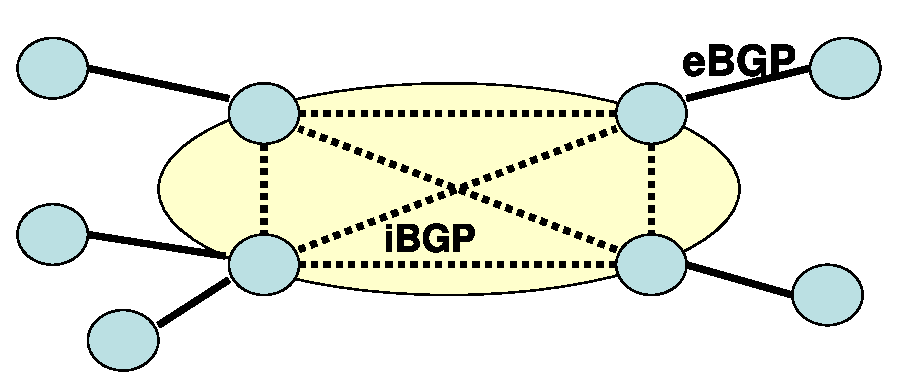
\epsfig{file=figures/pre_rcp.eps, width=0.45\linewidth}}\hfill
\subfigure[RCP receives the iBGP routes and the IGP topology from the
routers in the AS and computes routes on behalf of every router in the
AS, and assigns those routes using
iBGP~\cite{feamster:fdna2004}.]{ 
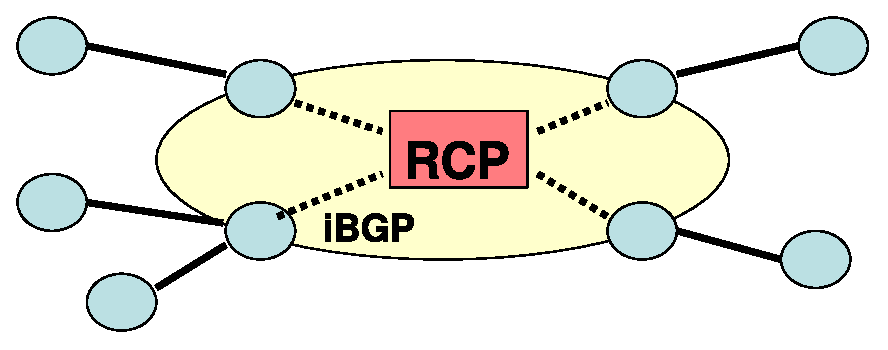
\epsfig{file=figures/rcp.eps, width=0.45\linewidth}}
\caption[Overview of Routing Control Platform]{Overview of the Routing
Control Platform (RCP) architecture.}
\label{fig:rcp}
\end{figure}

Rather than modifying the deployed routing infrastructure, the functions
of Internet routing could reside in a separate system that gathers
information about the topology (\eg, via iBGP and IGP), computes the
route that each router should use on behalf of each router, and assigns
the appropriate route to each router.  The idea of having a control
system that is separate from the infrastructure that is responsible for
forwarding packets (\ie, the routers) is the central idea of the 
Routing Control Platform (RCP)~\cite{caesar2004,feamster:fdna2004}
(see Figure~\ref{fig:rcp}), as well as work on a ``more versatile
route reflector'' that computes different routing decisions on behalf of
its client routers~\cite{id-versatile-rr}.  The IETF ForCES working
group has also proposed a framework that separates an individual
network element into separate control and forwarding elements, which can
communicate over a variety of media (\eg, a backplane, Ethernet,
etc.)~\cite{forces-wg}.  The framework dictates that routing protocols
be implemented in the control elements~\cite{rfc3746}.

Because RCP has a view of the AS-wide iBGP and IGP topologies, it can
assign routes to each router in a way that guarantees that the routing
protocol satisfies various properties, such as those from the
correctness specification in Chapter~\ref{chap:rlogic}.  RCP may also
simplify routing configuration, because configuration can be done on an
AS-wide basis, rather than router-by-router.  Rather than implementing
these policies with specifications of mechanism that are distributed
across the routers themselves, RCP could allow an operator to specify a
policy {\em for the entire AS} and be agnostic to the mechanisms that
actually implement the policy on the routers themselves.  

Separating routing state from the routers can potentially introduce
additional robustness, scalability, speed, and consistency problems.  The RCP
architecture must address these challenges to be viable.  We have implemented
a preliminary prototype of RCP as an 
extension to Quagga~\cite{www-quagga} to examine the feasibility of
having RCP control route selection for all of the routers in a large
tier-1 ISP~\cite{caesar2004}.  To study the other feasibility issues, we
are presently implementing RCP as extensions to the XORP software
router~\cite{Handley2002}; we plan to make this prototype available to
the research community.

%\section{Preventing Faults in the First Place}\label{sec:rcp}
%
%%%%
%%% introduction.tex
%%%

%\subsection{Introduction}\label{sec:intro}



Internet routing protocol
functionality should be separated from the routers.  Stated somewhat glibly,
routing is too important and too complicated to be
left to today's routers!  IP ``routers'' should be
``lookup-and-forward'' switches, forwarding packets as rapidly as
possible without being concerned about path selection.  
A separate entity should be responsible for 
computing the best BGP paths on behalf 
of all the routers in a domain and disseminating the results to the
routers. 

%Routers should forward packets but should not be
%concerned with distributed path computation.  Rather, a single
%logically centralized entity should perform all route computation on
%behalf of the routers in a routing domain.


%%%% This para should say WHY we believe in our position (motivation)

Separating interdomain routing from the individual routers is one way to
cope with the increasing complexity of the routing system.
The growth of the Internet has introduced considerable complexity into
interdomain routing, as  
features have been added to BGP to support
more flexibility (\eg, new route attributes such as communities and
MED) and larger scale (\eg, route reflectors and route aggregation).
This complexity has made routing protocol
behavior increasingly unpredictable and error prone~\cite{Feamster2004h}.
Requiring the 
routers to perform complex path computation introduces the potential
for inconsistencies across routers, complicates the expression of
routing policy, and makes troubleshooting difficult.


\begin{figure}[t]
\centering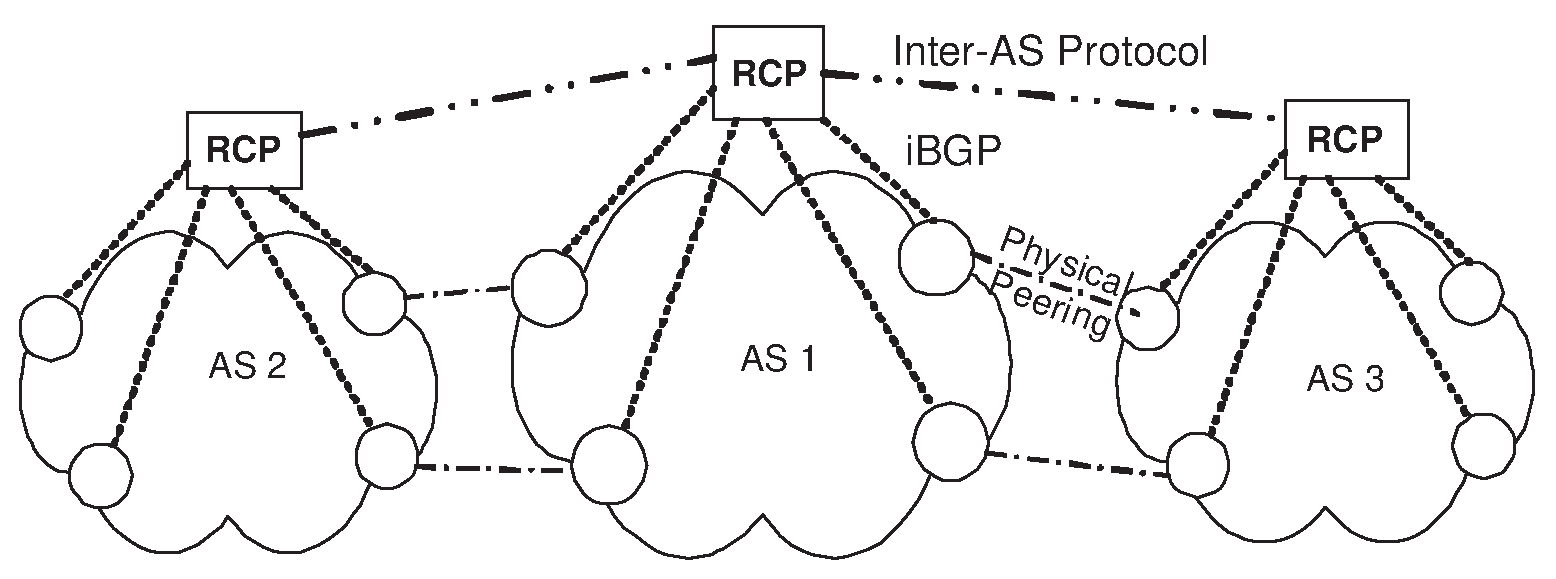
\epsfig{file=rcp/figures/interas.eps, width=\linewidth}
\caption[A Routing Control Platform (RCP) for the Internet.]{A Routing
Control Platform (RCP) for the Internet.  Circles 
  represent conventional routers.}
\label{fig:interas}
\end{figure}

%%% 
%%% Enabling 
%%%
Instead, a separate {\em Routing Control Platform (RCP)} should have
the information needed to select routes for each router in a domain
(\eg, an AS) and exchange routing information with RCPs in other
domains.\footnote{We use the term ``RCP'' to refer to
both the architecture as a whole and to the specific instance of RCP
within a routing domain.}
Figure~\ref{fig:interas} illustrates this idea.
%The RCP exchanges routing information with other ASes and sends each
%router in the AS a route to use in constructing its local forwarding
%table.  
Each RCP could use a new way of selecting routes for each router
(rather than using today's unwieldy BGP decision process); RCPs 
could even exchange routes using an interdomain routing protocol other
than BGP.  By selecting routes on behalf of {\em all\/} routers in a
domain, RCP can avoid many internal BGP-related complications (\eg,
forwarding loops~\cite{Dube99} and signaling partitions~\cite{Feamster2004h}).
%
%We believe that separating interdomain routing functionality from
%individual routers will reduce the complexity of routing configuration
%and management.  
%In this paper, we will
%describe how a logically centralized 
This approach also facilitates traffic engineering, simpler and less
error-prone policy expression, more powerful diagnosis and
troubleshooting, more rapid deployment of protocol modifications and
features, enforceable consistency of routes, and verifiable
correctness properties.  
%
In contrast to previous approaches for centralizing interdomain routes
and policies at route servers~\cite{Govindan1998}, RCP also preserves
the autonomy of each AS for selecting paths and applying
policies.\footnote{RCP more closely resembles the
Network Control Point (NCP), introduced in the telephone network in the
early 1980s to simplify network management and support the rapid
introduction of new features (\eg, enhanced 1-800 service)~\cite{Horing82,Lawser82}.}

RCP's deployment path is as interesting
as the envisioned end state.  The deployment of RCP can proceed in
three stages, offering the following benefits to network operators as
RCP becomes more widely deployed:

\begin{enumerate}
\itemsep=-1pt
\item \textbf{Control over protocol interactions:} RCP customizes the
distribution of BGP routes within an AS by replacing internal BGP route
reflectors.  This stage does not require cooperation from
neighboring domains.  Because RCP has a complete view of the intra-AS
topology and selects routes on behalf of all routers in the domain, it
can prevent internal BGP routing anomalies and control 
traffic flow more directly.

\item \textbf{Network-wide path selection and policy:} By establishing
BGP sessions
directly with the routers in neighboring ASes, RCP can perform all
routing decisions for an AS, bypassing the BGP decision
process on the routers.  This approach simplifies configuration and allows an
AS to select routes based on high-level goals, rather than obscure
manipulation of BGP route attributes.

\item \textbf{Redefinition of inter-AS routing:} Using RCPs, rather than
routers, to exchange routes between ASes (as shown in
Figure~\ref{fig:interas}) enables the design of a new routing protocol
because interdomain routing is now separated from IP routers.  For
example, RCP can be used to implement a control overlay that selects
paths based on prices or performance statistics.
\end{enumerate}
\noindent
%% Each phase reduces management complexity
%% fosters innovation and is completely backwards compatible with existing
%% routers. 


In addition to providing substantial improvements over today's routing
architecture, RCP has a compelling deployment incentive (\ie, a
``tipping point''), so that an individual AS could deploy RCP and
still realize significant benefits.  Because the first two stages of
deployment substantially reduce management complexity for BGP routing
{\em within a single AS\/}, network operators have a compelling
incentive to deploy RCP regardless of whether other ASes do so.
%Many innovative ideas (\eg, QoS, multicast, IPv6) have not yet
%been widely deployed operational networks because deploying these
%services provides no return until other ASes also do so.
%We believe that effecting real change in
%the Internet routing architecture requires a ``tipping point''---a
%compelling incentive for an AS to migrate to a new approach
%independently of other ASes.
%%%
%%% Tipping point
%%%
%Routing within a large backbone network depends on external BGP (eBGP)
%to exchange routes with other ASes, internal BGP (iBGP) to propagate
%these routes inside the AS, and the IGP to select paths between the
%routers in the AS.
Managing routing configuration requires constant vigilance from
network operators.  Although network management systems can often
automate the most frequent tasks, working around and within the
constraints of the existing routing protocols makes these systems much
more complicated than necessary.  Additionally, the complexity of
modeling and managing the distributed configuration state in today's
routers has itself impeded the evolution of automated management
systems.  
%Simplifying the management of a single network provides an
%incentive for an AS to deploy RCP independently of other ASes.
%%%
%%% As few changes as possible
%%%
In addition, because it communicates routes to each router in the
AS using BGP, RCP is backwards compatible with existing routers; deploying
RCP requires no changes to router hardware and software, only to
router {\em configuration}.


%%%%
%%% strawman.tex
%%%


\subsection{Architectural Principles for Routing}\label{sec:principles}

%% In this subsection, we describe the challenges of managing BGP within a
%% backbone network. Managing intra-AS routing presents three primary
%% challenges: (1)~the outcome intra-AS routing
%% depends on interactions between multiple routing protocols,
%% (2)~operators have indirect control over BGP's behavior, and (3)~because
%% iBGP's routing decisions are decentralized, common network management
%% and diagnosis tasks become more difficult.  The rest of this subsection
%% surveys these problems in further detail.

%% Despite the aspects of BGP that introduce fundamental problems and
%% stifle innovation, little attention has focused on designing protocol
%% improvements that fix these problems.  This lack of attention is largely
%% due to the fact that today's routing architecture does not support
%% innovation.  In this subsection, we describe three architectural principles
%% that will help facilitate innovation in interdomain routing.  In the
%% process, we describe specific aspects of today's routing system that
%% violate these principles.

In this subsection, we present three architectural principles for
reducing interdomain routing complexity:

\begin{enumerate}
\itemsep=-1pt
% 1
\item The routing architecture must base its routing assignments
on a consistent view of routing state. 
% 2
\item The interfaces between the routing protocols must minimize
unexpected or unwanted interactions.
% 3
\item The interdomain routing mechanisms must
directly support flexible, expressive policies.
\end{enumerate}
Each paragraph in this subsection discusses one of these principles.
For each principle, we present a high-level rationale, followed
by specific examples of how today's interdomain routing architecture
violates the principle.  For each of these examples, we suggest how
adhering to the architectural principle helps solve the problem.

%% In this subsection, we propose several architectural principles for
%% interdomain routing, all of which are rooted in traditional systems
%% design arguments, with the following goals in mind: (1)~to enable
%% innovation by fostering a more open platform for interdomain routing;
%% and (2)~to mitigate complexity of the interdomain routing system in
%% order to make network management easier.  To make the deployment of an
%% extensible routing platform feasible, we must keep both
%% goals in mind; in particular, the latter goal is the ``tipping point''
%% that gives operators an incentive to deploy an architecture based on
%% these principles.

\paragraph{Compute Routes Using Consistent State}

Routing state and logic should be co-located with the system components
that are assigning routes.  The logical participants in an interdomain
routing protocol are the {\em ASes\/}, not the individual routers.  The
interdomain routing architecture should view each AS as a single
participant and base routing decisions on a network-wide view of
available routes and configuration state; the routers, on the other
hand, should forward data traffic without concern about how the routes
are computed.  The current interdomain routing system violates this
architectural principle in the following three ways:
%
%The network ``core'' should maintain as little state as possible and the
%intelligence in networks should exist at endpoints.  
%Although the original Internet routing architecture incorporated the
%spirit of the end-to-end argument, 

%This argument holds
%important lessons for interdomain routing.  
%Routing is a distributed program that assigns IP-level paths to each
%destination.  


%First, {\em placing the ``intelligence'' of the routing protocol in
%the routers themselves prevents experimentation with and rapid
%deployment of new features}.  Many of the features of the interdomain
%routing system have ended up in the hands of router vendors because,
%to date, the best (and, arguably, the only) place to add functionality
%to the network is in the routers themselves.  Unfortunately, because
%most innovation at the routing layer involves compliance with
%proprietary hardware and software, as well as the slow-moving
%standards process, innovations to the routing architecture have been
%incremental and difficult to deploy.  Router vendors often add
%functionality in response to requests for new features (such as
%route-flap damping or BGP communities).  Moving the routing protocol
%logic out of the routers to the extent possible would allow protocol
%designers and network operators to easily experiment with and quickly
%deploy protocol modifications, without being tied to router hardware
%and software development cycles.

{\bf Decomposing the routing configuration state across the routers
unnecessarily complicates policy expression}.  Although
distributing state to achieve scalability and reliability makes sense,
many aspects of configuration are not replicated, but rather {\em
decomposed} across routers.  
%This decomposition
%of policy across routers does not improve scalability or reliability,
%but complicates policy expression and makes configuration
%inconsistencies more likely.  
Configuration state should be logically
centralized because it simplifies policy expression without compromising
scalability or reliability.

\vspace{0.05in}
\noindent
{\em Problem:} Network operators must often implement high-level policies,
such as preventing routes learned from one AS from being advertised to
another.  Implementing this policy currently requires modifying the
configurations of multiple routers: the import policies must ``tag''
eBGP-learned routes appropriately, and the export policies of other
routers must filter routes with this tag when advertising to eBGP
neighbors.  

\vspace{0.05in}
\noindent
{\em Solution:} Defining routing policy on a network-wide basis would
obviate the need for this level of indirection.  A network-wide
configuration management entity could know the origin of all routes
based on the eBGP sessions that advertised them, which would allow
a direct expression of policies based on sessions.
\vspace{0.05in}

%Because complexity makes reasoning extremely
%difficult, operators may be less likely to modify configuration because
%they lack the ability to reason about high-level behavior and fear
%introducing mistakes into the configuration.
%Additionally, distributing configuration can introduce
%unnecessary dependencies that actually make the routing protocol more
%error-prone than it should be.  
%This complexity discourages makes operators reluctant to experiment with
%changes and improvements for fear of introducing unintended side effects
%or ``fixing something that isn't broken''.  
%Configuration state should
%be distributed when doing so enhances scalability or reliability;

{\bf Distributed path selection causes routing decisions at one router
  to depend on the configuration of other routers}.  Subtle
  configuration details
  affect the route that a router selects or whether that router learns a
  route at all.  Computing routes on a network-wide basis using a
  consistent view of routing state can reduce interdomain routing's
  dependencies on these subtle details.
%selection can both explicitly enforce correct operation and facilitate
%modeling of the protocol behavior.
%

\vspace{0.05in}
\noindent
{\em Problem:} 
Omitting a single iBGP
session in a full-mesh configuration can leave a router with no route
for certain destinations, even if the intradomain topology is connected.
Distributed path selection also makes 
predicting the effects of configuration changes on traffic
flow difficult~\cite{Feamster2004}. 

\vspace{0.05in}
\noindent
{\em Solution:} 
An entity that performs path assignment on behalf of all
routers could control path assignment to ensure that every router is
assigned a route for every destination.
%For example, consider
%Figure~\ref{fig:today}, which shows how eBGP, iBGP, and IGP
%interoperate.  A router that learns a route on an iBGP session will not
%readvertise that route to routers on other iBGP sessions because those
%routers should have heard the same route from the router that learned
%the route via eBGP; if the iBGP topology is configured such that the
%routers in the top-level of the route reflector are not fully meshed,
%iBGP may not propagate routes to every router in the AS.
%(Incorrect iBGP configuration can also cause routing loops and
%oscillations; we discuss this in Section~\ref{sec:layer}.) 
\vspace{0.05in}

{\bf Each router is unaware of the state at other routers; this lack of
  information may result in incorrect or suboptimal routing.}.
  Implementing BGP's many features on the routers makes these features
  difficult to reason about.  For example, replication of functionality
  that is intended to
  improve reliability can cause forwarding loops, and a feature intended
  to prevent routing instability can slow convergence.  A routing
  architecture should implement these features in a 
  module that has
  a complete view of the network state, rather than in the routers
  (each of which only has a partial view of network state); doing so
  would allow that module to ensure sensible, consistent network-wide
  route assignment and override any feature interactions that cause
  incorrect routing. 
%  Controlling these protocol interactions centrally also makes it much
%  easier to physically replicate the entity performing route
%  computation.

%
% route-flap damping
\vspace{0.05in}
\noindent
{\em Problems:} 
% MED
%As another example, BGP's MED attribute allows an AS to express
%preference for how its neighbor selects an egress point for sending
%traffic (\ie, ``cold-potato'' routing).  Because MEDs are
%compared only between routes learned from the same AS, a router cannot
%form a total ordering of routes, which can cause persistent route
%oscillation~\cite{Griffin2002}.
% RR replicas
A router typically has iBGP sessions to multiple
route reflectors to improve reliability.  When a route reflector
fails, protocol oscillation and forwarding loops can arise if the
second route reflector has a different view of the best routes.
Placing the two route reflectors close to each other reduces these
kinds of inconsistencies but introduces fate sharing (\ie, the risk of
shared failures). 
%On the other hand, we believe that 
As another example, BGP route flap damping suppresses
unstable routes that change frequently~\cite{rfc2439}.  Unfortunately,
sometimes a 
single failure can trigger many advertisements that can mistakenly
activate route flap damping~\cite{Mao2002}.  Network operators must work
backwards to select configuration parameters that prevent erroneous
damping.

\vspace{0.05in}
\noindent
{\em Solution:} 
An entity that performs route
computation using a consistent view of available routes and network
topology can be replicated using standard distributed 
systems algorithms. Unlike route reflectors, each replica would assign
the same route to each router, independently of its location in the
network.
A module with knowledge of the routes assigned to every router in the
AS could also detect when route changes are caused by path exploration and
avoid unnecessarily suppressing a route.

\vspace{0.05in}
%Whenever possible, routing-protocol functionality should be decoupled
%from the routers.  That is there is no fundamental reason why a
%separate, vendor-independent device could not choose paths on behalf
%of the routers.  We believe that much of the research community's
%affection for overlay networks comes from the desire to control
%Internet routing and the frustration that the IP routing architecture
%remains largely closed to innovation.  Separating the path-selection
%process from the routers would enable exactly the kind of
%experimentation enabled by overlays today, but with the hope of
%directly influencing the behavior of the {\em underlay\/} network.

%%XXX Mention vendor-specific configuration? XXX

%Allowing each router in the AS to perform path selection introduces a
%A participant in a dynamic routing protocol updates its path selection
%as available routes change.
%If the routing decisions at each router are coupled with
%the propagation of the routing messages themselves, inconsistent (and
%incorrect) paths can result as updates propagate.  

\paragraph{Control Routing Protocol Interaction}\label{sec:layer}

Dividing functionality into distinct modules with clear interfaces can
control complexity.  In the routing system, the {\em IGP\/} computes
paths between routers in an AS, {\em eBGP\/} computes paths between ASes,
and {\em iBGP\/} propagates eBGP-learned routes throughout an
AS.  At a higher 
layer, {\em overlay networks\/} route traffic along one or more end-host
hops, abstracting the IP substrate entirely.
%In this subsection, we argue that the process of network protocol design
%and operation should respect this layering.
%
%As shown in Figure~\ref{fig:today}, an AS's border routers use eBGP to
%exchange routes for global destinations with other ASes; we call the
%layer at which eBGP routes are exchanged the {\em eBGP layer}.  Each
%eBGP-speaking router uses iBGP to exchange routes for global
%destinations with other routers in its AS.  We will refer to the layer
%at which iBGP routes are exchanged the {\em iBGP layer}.  If one of
%these routers selects a route for some destination that it learned from
%another router via iBGP, it will forward packets for that destination to
%that other router using the IGP path.  We will refer to the layer at
%which routers forward packets within an AS as the {\em IGP layer}.
%
Unfortunately, the modules in today's
interdomain routing system interact in the following undesirable ways:

{\bf Hard-wired interactions between eBGP and the IGP constrain an
operator's control over path selection.}  Although the internal
topology should have some influence on BGP routing decisions (\eg, 
it allows nearest-exit routing), a
router's choice of egress point should be relatively insensitive to
small IGP changes.
%, but it should still use IGP
%information when it informs BGP route selection.
%% Although the
%% routing architecture should {\em enable\/} IGP path costs to influence
%% the BGP routing decision, the interaction between the IGP and eBGP
%% layers {\em should not be hard-wired\/}.
%A router may learn multiple routes to a destination over several iBGP 
%sessions.  That router then applies a {\em de facto}
%``decision process'' to select a single best route to a destination.
%One step in that decision process dictates that routes with lower cost
%IGP paths be preferred over routes with longer IGP paths to an exit
%point.  
%The interplay between BGP and IGP limits operator control in two ways:
%(1)~minor changes in IGP routing can cause disproportionate effects in
%BGP routing, and (2)~to effect changes in intra-AS routing for network
%engineering, network operators are often forced to adjust the interdomain
%protocol configuration.
%
%Despite the benefits of hot-potato routing, 
%This happens because the BGP path selection process introduces
%dependencies on the IGP, a layering violation.

\vspace{0.05in}
\noindent
{\em Problem:} 
The BGP decision process uses the IGP path cost to break
the tie between two ``equally good'' routes. Internal events, such as
link failures, planned maintenance, or traffic engineering often lead to
changes in the IGP path costs.  These IGP changes can cause a router to
change its best {\em BGP\/} route, causing abrupt, unwanted traffic
shifts~\cite{teixeira2004b}.  Additionally, an operator may sometimes {\em
want\/} to redirect traffic from one egress link to another.  Today,
this requires complex manipulation of the BGP import policies to make
some egress points less attractive than others~\cite{Feamster2003e}.

\vspace{0.05in}
\noindent
{\em Solution:} 
With better control over the interactions between eBGP and IGP, an
operator could directly assign new routes to some routers without changing
BGP routing policies.
\vspace{0.05in}

{\bf Inconsistencies between iBGP and IGP can cause
forwarding loops and route oscillation.}  Operators can test that
their iBGP configuration satisfies sufficient conditions for
correctness~\cite{Griffin2002}, but this 
approach is not robust because operators commonly misconfigure
iBGP~\cite{Feamster2004h}.  The routing architecture should
explicitly {\em enforce\/} correctness constraints.  

\vspace{0.05in}
\noindent
{\em Problem:}
An
iBGP route reflector selects and distributes one best BGP route for each
destination prefix.  As a result, the route-reflector clients do not
necessarily make the same BGP routing decisions as they would in a
full-mesh iBGP configuration.  In particular, a route reflector and
its clients may have different IGP path costs to the
egress routers, leading to different BGP routing decisions, as shown 
previously in Figure~\ref{fig:rr}. 
%A route reflector and its clients may have a different view of the IGP
%path costs, which could result in inconsistent paths to the same
%egress point.
These inconsistencies can lead to protocol oscillations or persistent
forwarding loops~\cite{Basu2002,Griffin2002,rfc3345} if a router
forwards a packet toward one egress point via a router that has
selected a BGP route with a {\em different} egress point.  These
``deflections'' can also cause the AS-level forwarding path to differ
from the BGP AS path, which can complicate debugging~\cite{Mao2003}.

\vspace{0.05in}
\noindent
{\em Solution:} 
Rather than being agnostic about IGP forwarding paths, the routing
architecture could use the available knowledge to explicitly enforce
consistency in router-level forwarding paths.
\vspace{0.05in}

%decision process, can cause persistent route oscillation if route
%reflectors and their clients are not configured
%correctly~\cite{Griffin2002b,rfc3345}.  Griffin {\em
%et al.} observed that iBGP and IGP suffer from {\em asymmetry}, where
%the path over which data travels (determined by the IGP) is not
%necessarily the reverse of the control traffic
%(determined by the iBGP signaling graph)~\cite{Griffin2002}.  Asymmetry
%between iBGP and IGP can cause loops or ``deflections'' (\ie, instances
%where the forwarding path does not match the path indicated by the
%corresponding route), because routers along the IGP
%path may not agree on the same route to a
%destination~\cite{Dube99,Griffin2002}. 

%The interactions between iBGP and IGP complicate route selection and
%router-level forwarding paths. Even if an operator could predict the
%route that each router selects for a destination, it is still often
%difficult to determine whether the path over which packets are forwarded
%will actually follow that route.  For example, although conventional
%wisdom holds that iBGP route reflection simulates the effects of a full
%mesh iBGP topology, route reflection does not in fact do this.  A route
%reflector effectively executes the BGP decision process on behalf of its
%clients {\em under the assumption that its clients would have selected
%the same best route}.  Thus, the route that a router selects depends on
%the configuration of the route reflector hierarchy.  Configuring the
%route reflector hierarchy to avoid persistent forwarding loops requires
%extreme care.
%
%Although following proposed configuration guidelines can mitigate the
%undesirable interactions between iBGP and IGP, these work\-arounds
%avoid the fundamental protocol design problems that must be addressed as
%part of a long-term solution.  Interactions between iBGP and IGP become
%more considerably complex as the number of routers in an AS increases.
%One way of mitigating this complexity is to divide a large AS into
%multiple smaller ASes (or ``confederations'') with fewer routers.
%However, each configuration must still use iBGP to propagate routes
%internally, and the resulting larger network now comprises multiple ASes
%which are subject to misconfigurations themselves.  Additionally,
%previous work has derived sufficient conditions that must exist for iBGP
%to converge to a stable, loop-free routing that correctly propagates
%routes~\cite{Griffin2002}, but the protocol does not explicitly enforce
%these conditions.
%Although this work
%presents a practical, immediate way to avoid certain iBGP correctness
%problems, 
%the sufficient conditions on routing configuration are merely
%The intra-AS routing protocol should be designed to {\em
%enforce} these correctness constraints and explicitly prevent unwanted
%interactions between routing layers.\footnote{Tunneling (expand this)
%(\eg, via MPLS or IP-in-IP encapsulation) prevents persistent
%forwarding loops because forwarding decisions within the AS are
%determined by tunnels, rather than destination-based routing.
%Essentially, this type of tunneling enforces a layer separation between
%iBGP and the intra-AS routing. XXX Doesn't solve everything.}

{\bf Interactions between overlay networks and the underlying
network can degrade performance}.  
Overlay networks measure end-to-end path performance and tune routing
at the edge of the network, but they typically lack (1)~detailed {\em
measurements\/} of traffic and routing that would help them make
better decisions and (2)~direct {\em control\/} over IP-layer
protocols and mechanisms. The routing architecture should provide the
information and control that overlays need via a well-defined
interface. 
%

\vspace{0.05in}
\noindent
{\em Problem:} 
Route control products~\cite{www-routescience,www-sockeye}
help multihomed ISPs select upstream routes for each destination,
whereas end-host overlays such as RON~\cite{Andersen01} circumvent
failures and congestion by directing traffic through an intermediate
host.
% why are they harmful
Because they lack complete information about routing and
traffic-engineering optimizations, these overlays sometimes increase
congestion and decrease the effectiveness of traffic engineering in the
underlay network~\cite{Qiu2003}, which can degrade user performance.

\vspace{0.05in}
\noindent
{\em Solution:} 
With more direct control, overlays could operate more efficiently (\eg,
by not sending the same traffic over congested links at the network
edge~\cite{Jannotti2002}).  With more information about routing
dynamics, overlays could
pre-emptively avoid some outages~\cite{Feamster2003}. 

%% A control overlay, with a node in each AS, could monitor the behavior of
%% the routing system and drive the selection of paths in the under
%% network.  With an appropriate interface, this control overlay could
%% provide invaluable support to conventional overlay networks.


%Overlays improve end-to-end path performance and increase routing
%flexibility, but giving overlays the appropriate interface to the IP
%layer can improve network performance further.  Rather than creating
%control loop interactions between overlays and IP routing, the network
%architecture could provide the overlay with some level of control over
%the IP layer path to a destination.  Conversely, the IP layer could
%take ``hints'' from the overlay about end-to-end path performance and
%incorporate this into path selection at the IP layer.


% {\em BGP confederations or separate ASes:} problem still exists in
%      each confederation or mini-AS (though maybe RRs can be avoided), and
%      you now have to model a multi-AS network.  (I need to read ``on being
%      the right size'').




\paragraph{Support Flexible, Expressive Policies}

%% <<<<<<< strawman.tex
%% When used appropriately, abstraction can mitigate the complexity in
%% complex systems.  

%% However, the indirection that interdomain routing employs actually
%% exposes complexity rather than hiding it.  BGP's configuration and
%% operation involves multiple levels of indirection, but the indirection
%% it uses serves to complicate the protocol by {\em exposing mechanism},
%% rather than abstracting these details.  An interdomain routing protocol
%% should allow operators to specify tasks at the appropriate level of
%% abstraction, in a way that hides the mechanistic details of the routing
%% protocol rather than exposing them.  Note that these problems are not
%% merely configuration problems but involve fundamental protocol design
%% principles.
%% =======

%Much of the complexity of interdomain routing comes from the need to
%support competing domains with complex, sometimes conflicting, policy
%goals.  In fact, 
The interdomain routing architecture must support flexible, expressive
policy.  The need for greater flexibility in selecting and exporting
routes has driven many of the extensions to BGP over the past fifteen
years, and we believe this trend is likely to continue.  Although BGP is
highly configurable, its operation is controlled by {\em indirect\/}
mechanisms that expose details rather than abstracting them.
Architectural simplifications and better abstractions can simplify
configuration languages and make policy specification simpler and more
expressive.  The following points illustrate why today's routing
architecture does not satisfy these goals:

%Complex systems often exhibit emergent properties and unintended side
%effects. For example, a feature that is added for a certain reason may
%interact with others in strange and unexpected ways.  To control these
%types of effects, system designers often apply {\em modularity}:
%dividing the components of a system into groups of components such that
%each group can be reasoned about independently.  Designers aim to divide
%a system into modules in a way that minimizes the number of
%interconnections between modules.  Modules then interact with each other
%and with the environment via well-defined interfaces.  BGP's design
%gives rise to feature interactions, unnecessarily exacerbating
%complexity.  BGP's configuration and operation involves multiple
%unnecessary levels of indirection, which complicate the protocol by {\em
%exposing mechanism}, rather than abstracting these details.  In the
%remainder of this subsection, we describe how BGP's design restricts
%flexibility and gives rise to complicated feature interactions.

{\bf BGP's mechanisms preclude the expression of certain policies
and make others difficult to express.}  Network operators influence the
outcome of the BGP decision process by configuring policies that modify
the attributes of BGP routes.  Better configuration languages would be
helpful, but the architecture should also provide more flexible support
for assigning paths to routers.  

\vspace{0.05in}
\noindent
{\em Problem:} 
Moving
traffic from one inter-AS link to another requires~\cite{Feamster2003e}:
(1)~identifying the subset of prefixes that carries the desired amount of
traffic, (2)~determining how to express that subset (\eg, by a common
AS path regular expression), (3)~modifying the import policies on one or
more routers to assign a smaller ``local preference'' for routes
matching those expressions, and (4)~observing the resulting traffic flow
and iterating as necessary.  

\vspace{0.05in}
\noindent
{\em Solution:} 
Although ``what if'' tools can help predict
the effects of policy changes~\cite{Feamster2004}, the routing architecture
should allow an operator to move traffic by {\em explicitly} assigning paths.

%% Additionally, BGP has a ``hold timer'' setting that
%% specifies how the router will wait in between BGP ``keepalive'' messages
%% before deciding that a session has failed.  The hold timer setting is an
%% indirect mechanism for expressing how fast a router should detect a
%% failure.  The setting of the hold timer is somewhat of an art: for
%% example, a short hold timer interval allows for quicker detection of
%% failed sessions, but the interval must be longer than IGP convergence
%% delay to prevent spurious session resets.

{\bf BGP's mechanisms impede multiple ASes from cooperating in
selecting routes that satisfy their goals.}  ASes must cooperate to
ensure end-to-end reachability, but today's routing architecture does
not directly support this type of cooperation.  Interdomain routing
policies are a tussle space~\cite{clark2002}: an AS must balance the
dependence on its neighbors for good connectivity to the rest of the
Internet and competition with neighbors for customers and revenue.
Operators must currently resolve these conflicts outside of the
infrastructure, but
the architecture should directly support route
selection based on negotiated preferences or financial incentives.

\vspace{0.05in}
\noindent
{\em Problem:} 
Suppose one AS wants to advertise a backup route to its
neighbor.  These two ASes must first negotiate a backup
``signal'' out of band.  The AS advertising the route must then modify
its export policies to attach this signal to the backup route, and the
neighbor must modify the import policies on its routers to lower
the ``local preference'' value for routes with this community.

\vspace{0.05in}
\noindent
{\em Solution:} 
Because route negotiation is fundamental to inter-AS
cooperation, the interdomain routing should support it directly. 

%Additionally, an
%upstream neighbor might have a strong preference for the second route
%but would not have an easy way to convey this interest.  Although such
%preferences could be conveyed out of band~\cite{mahajan2005}, each AS
%would need to reconfigure each router appropriately.


%% Finally, {\em router configuration languages dictate low-level
%% specification of protocol behavior, rather than high-level policy or
%% operator intent}.  Operators must express constraints on route
%% distribution using indirect methods of expression.  To do so, they
%% typically implement filters that control the distribution of routes
%% based on whether a route's attributes matches specified pattern.  For
%% example, an operator may configure a router to filter routes that have a
%% certain ``community'' attribute~\cite{rfc2519}.  Controlling route
%% propagation using communities involves definitions at three levels of
%% indirection: (1)~mapping a BGP session to the names of import and export
%% policies, (2)~mapping the name of each policy to a set of clauses, each
%% of which defines conditions for accepting or rejecting a route and
%% modifying route attributes, and (3)~defining various variables that are
%% used in the clause of a policy statement (\eg, specifying what AS
%% regular expression number $x$ refers to).  These levels of indirection
%% make controlling route distribution complicated and error-prone because
%% they specify {\em how} the protocol should implement a certain behavior,
%% rather than directly specifying the policy to implement.  A
%% protocol and configuration language that supported direct expression of
%% high-level policy would ease the burden of network management.
%  communities+ACLs for aggregation~\cite{rfc2519}
%  and imposing relationships like customer, peer, and provider

%An interdomain routing protocol should allow operators to specify tasks
%at the appropriate level of abstraction, in a way that hides the
%mechanistic details of the routing protocol rather than exposing them.
%Note that these problems are not merely configuration problems but
%involve fundamental protocol design principles.  Better router
%configuration languages would mitigate some of these problems, but many
%of the problems associated with this interface result from incorrect
%{\em protocol} mechanisms.  Thus, allowing operators to configure
%routers at the appropriate level of abstraction involves architectural
%changes, as well as improvements to the configuration language itself.







%\subsection{Routing Control Platform (RCP)}\label{sec:arch}
Building on the principles from Section~\ref{sec:principles}, this
subsection proposes a {\em Routing Control Platform} (RCP), which
separates the control-plane logic from the routers that forward packets.
We describe RCP as a single, logically-centralized entity in each
domain. This centralized function must actually be implemented in a
reliable, physically distributed fashion to avoid introducing a single
point of failure and ensuring robust route distribution.  We believe
that existing distributed systems techniques may be applicable; this
dissertation does not address this issue in detail, but we briefly
discuss it in Section~\ref{sec:weaknesses}.

We describe RCP in terms of three phases: (1) controlling routing
protocol interactions by replacing iBGP route reflection with RCP, (2)
gaining flexibility over route selection by making RCP the
endpoint of all eBGP sessions with neighboring ASes, and (3) enabling
changes to interdomain routing by using RCPs, rather than routers, to
exchange routes between ASes using eBGP or some new protocol.
%
By describing RCP in terms of three stages, we demonstrate that RCP is
incrementally deployable {\em within an AS\/} and, more importantly,
provides significant benefits to an individual AS even if other ASes
have not deployed RCP.  In addition to being steps of incremental
deployment, each phase provides  new functionality while
remaining  backwards compatible with BGP.  
%RCP simplifies the
%operation of interdomain routing within individual ASes, regardless of
%whether other ASes deploy RCP. However, RCP's full potential is only
%realized when it is completely deployed by a group of interconnected
%ASes or throughout the entire Internet.
%The rest of this subsection describes these three modes of deployment in
%further detail.  For each stage, we describe the changes that must be
%made to the way that BGP is {\em configured}, as well as how each stage
%makes reduces complexity and enables innovation.
%Table~\ref{ref:phases} summarizes the architectural changes at each
%phase of evolution, as well as new features and functionality that are
%enabled at each phase.

%% \begin{figure}
%% \centering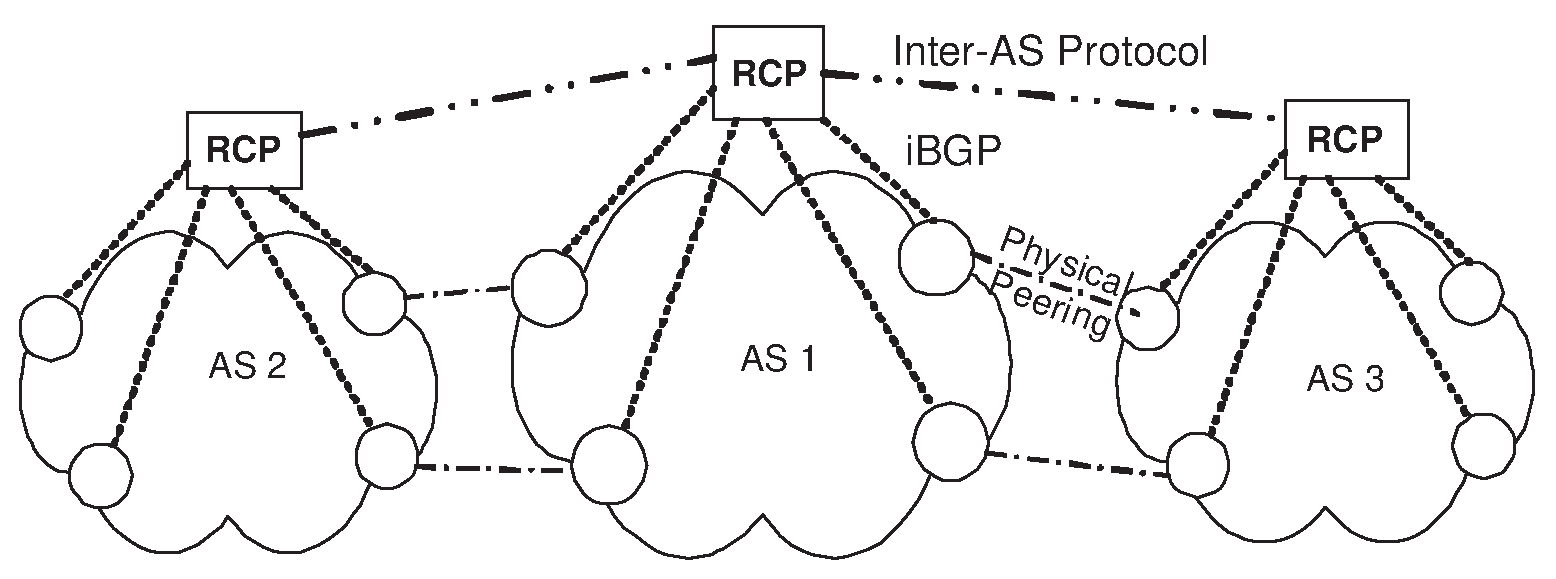
\epsfig{file=rcp/figures/interas.eps, width=\linewidth}
%% \caption{An extensible routing platform for the Internet.}
%% \label{fig:interas}
%% \end{figure}


%%%%%%%%%%%%%%%%%%%%%%%%%%%%%%%%%%%%%%%%%%%%%%%%%%%%%%%%%%%%

\paragraph{Control Over Protocol Interactions}\label{sec:feamster:fdna2004_ibgp}


%% note: already exists a monitoring infrastructure.  now we're going to
%% let the monitor "talk back" 
%% A route authority must have sufficient information about the state of
%% the network from the perspective of its clients to make the correct
%% decision for each client.  The route authority acts as a proxy for each
%% of its clients; thus, to make the same decision that the client would
%% have made in a full-mesh configuration, the authority must have access
%% to all of the information that the client would have used to make the
%% same routing decision in a full mesh (\eg, IGP path costs from that
%% client to a network egress point).

The first phase of RCP deployment, shown in Figure~\ref{fig:ibgp_only},
involves only minor changes to the iBGP {\em configuration\/} inside
an AS.  
% Monitoring the IGP
First, RCP monitors the IGP to
maintain an accurate, up-to-date view of the IGP topology; previous
work explains how to monitor an IGP without disrupting the operation
of the network~\cite{Shaikh2004}.
Next, instead of having routers propagate eBGP-learned routes through
an iBGP hierarchy, a router sends its best route for each eBGP-learned
destination to RCP via an
iBGP session.
% Making the decisions
Finally, RCP computes a route for each router and conveys that route via
the iBGP session. 
% It's not too bad
Using an RCP does not require any changes to the routers themselves
(aside from the configuration of iBGP sessions to RCP) or the
configuration of routers in other ASes.  Many ISPs already deploy a
monitoring infrastructure to keep track of network state and routing
protocol behavior.  At this stage, RCP is essentially an IGP and BGP monitoring
infrastructure that also {\em controls} route selection.


\begin{figure}
\centering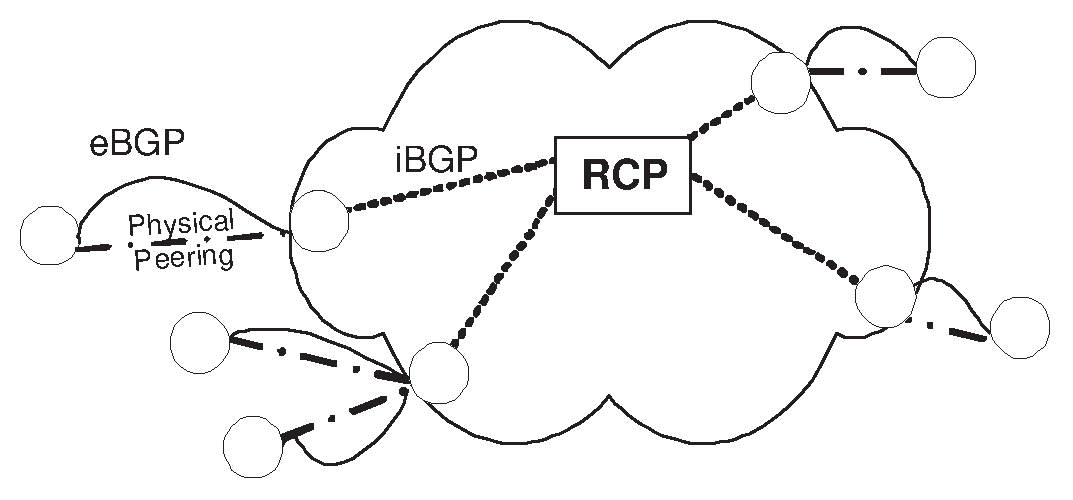
\epsfig{file=rcp/figures/ibgp.eps, width=0.6\linewidth}
\caption[The first phase of RCP deployment]{The first phase replaces the
pairwise iBGP sessions between  
routers with iBGP sessions to RCP.  RCP uses knowledge about the
IGP topology and the best routes from each border router to
make routing decisions on behalf of each router.  RCP distributes the
path assignment to the routers via iBGP.}
\label{fig:ibgp_only}
\end{figure}


This stage of RCP closely resembles an architecture based on route
reflection~\cite{rfc2796}, but, unlike route reflectors,
RCP can return a {\em different\/} best route to each router.  For
example, RCP could compute the route that each router would have
selected in a full-mesh iBGP topology.
%, which computes the same routes
%as a full-mesh configuration (unlike
%a route-reflector hierarchy).  
RCP also offers more
flexibility than route reflection because it is not
limited to emulating a full-mesh iBGP scenario: RCP could
intentionally select other routes to control the interactions between
iBGP and the IGP.
% not a route server
RCP may also appear similar to previous work on route
servers~\cite{rfc1863} that forward {\em all\/} BGP-learned routes to
their clients, but, because it forwards only {\em one\/} route to each
client, RCP remains backwards compatible with BGP and enables
customized path selection.

In the rest of this paragraph, we present several examples to 
show how this stage of RCP deployment simplifies important network
management tasks. 

{\bf Enforceable correctness constraints and invariants.}  With
complete knowledge of the iBGP and IGP topologies, RCP can 
enforce a clean separation of routing layers.  
%For example, as we pointed out in Section~\ref{sec:principles},
%interactions between iBGP and IGP can result in incorrect routing if
%certain sufficient conditions are not satisfied.  Currently, operators
%must check these conditions manually or with an external configuration
%checker~\cite{feamster03:verify}.  Of course, the RCP could examine
%the routing protocol configuration and check these sufficient
%conditions, but, because the RCP {{\em controls} the routing decisions
%for the routers in the AS, it can directly {\em enforce} correctness
%constraints.  For example, persistent forwarding loops can result if
%the routers along an IGP path do not select the same BGP
%route~\cite{Dube99}.
For example, RCP can ensure that each router along a forwarding
path selects the same best BGP route for a destination prefix, which
prevents the forwarding loops and protocol oscillations that 
can arise in conventional iBGP configurations~\cite{Dube99,Griffin2002}.
%
RCP can also be useful for detecting persistent oscillations caused by
the MED attribute~\cite{Griffin2002b}, which occurs because routers do
not have a total ordering over the set of candidate routes.  With a complete
view of the best routes from each border router, RCP can recognize
when each router would not have a single, consistent ordering and
can force the system into a stable path assignment. 

%% {\bf Improved routing during convergence.}  Because correct, loop-free
%% routing within an AS depends on consistency between iBGP and IGP routes,
%% forwarding loops can also result as a result of either iBGP or IGP
%% convergence.  For example, two routers may agree on an egress router for
%% a global destination.  If one of those routers hears a withdrawal for
%% that exit point before the other, the router that first hears the
%% withdrawal could select an alternate route that forwards packets towards
%% the router that has not yet heard the withdrawal and is still using the
%% old exit point.  Such a situation could cause unnecessary transient
%% forwarding loops during convergence.  By removing the complexity of
%% route propagation from the routers themselves (Principle~1), the RCP can
%% control the propagation convergence-related routing changes to minimize
%% these temporary inconsistencies.

{\bf Avoiding unintentional hot-potato routing changes.}  Small
changes in the IGP topology (\eg, due to traffic engineering,
failures, or planned maintenance) can trigger large, unnecessary
shifts in eBGP routes because of BGP's ``hot potato'' routing
behavior~\cite{teixeira2004b}.  RCP can allow a network operator to add
or remove internal links, or modify the IGP costs, without worrying
about the side effects on BGP path selection.  By controlling the path
selection for each router, RCP can force routers to continue using an
egress point even when a link failure or small IGP cost change makes
another egress point become slightly ``closer''.  (RCP must take care
to ensure that each router along the forwarding path to the egress
point for that router continues to pick the same egress point.)  In
addition to avoiding unnecessary traffic shifts,
% and BGP convergence delays within an AS, 
preventing these abrupt routing changes improves global
routing stability by reducing the number of eBGP routing changes
propagated to downstream neighbors.

{\bf More flexible traffic engineering.}  RCP can
{\em intentionally\/} change the egress point for a router to move
traffic to a lightly-loaded edge link or a less congested downstream
path.  This approach allows the AS to balance the traffic load without any
changes to the import policies on eBGP sessions or the IGP link costs.
In addition to controlling the egress point, RCP could
dictate the entire forwarding path through the AS rather
than relying on the IGP.  For example, RCP could send a router a
BGP route with a ``next hop'' that corresponds to an immediate
neighbor in the IGP topology, which would cause that router to create a
forwarding table entry that maps the destination prefix to the
outgoing link connecting directly to the neighboring router.  
This
kind of fine-grained control is useful for planned routing changes.
RCP could make these routing
changes incrementally (\ie, one router at a time) to avoid creating transient
forwarding loops during convergence.
%For example, the RCP could pin a fixed path through a sequence of
%routers in an AS by ensuring that those routers were always assigned
%the same exit point for a destination (exit-point tunneling).  If an
%AS already performs intra-AS routing with tunneling (\eg, with MPLS),
%RCP can simplify path selection further---once label distribution has
%established paths, RCP can distribute traffic flow across the AS
%simply by assigning labels at ingress routers.

%The RCP could also assign routes to a destination with the next-hop
%attribute for each router set to the next {\em intra-AS hop} within that
%AS, rather than to that of the exit point (intra-AS ``hop-by-hop'' routing).
%Using hop-by-hop routing with RCP has several advantages.  First,
%because the intra-AS path is explicitly encoded in the iBGP route, each
%iBGP hop can potentially be only a single IGP hop; this feature
%decouples iBGP and IGP.  Second, this decoupling makes traffic
%engineering and network management much more flexible, because operators
%can establish intra-AS paths using the RCP without worrying about how
%those paths will be affected with IGP paths change.

%% {\bf More expressive backup policies.}  Ability to express new policies,
%% such as those involving multihoming and backup (Rekhter's RFC on
%% multihoming and aggregation, ideas about failure detection/health
%% monitoring).  Something about health monitoring here; knowing when to punch
%% holes, etc. requires knowing whether the eBGP link has failed, or
%% whether some iBGP link has failed.


%% {\bf XXX should have an example here XXX} Each client should be able to
%% select the route that it would have selected in a full-mesh
%% configuration.  The route or routes that a client learns via the
%% intra-AS routing protocol should always include the route that the
%% client would have selected in a full-mesh iBGP configuration.  What
%% problems go away with tunneling?  Forwarding path inconsistencies {\em
%% only} (deflection and forwarding loops).  Rest of the problems remain.


%% There is a broad spectrum of possible solutions that could simulate a
%% full mesh, many of which would involve changing the format of routing
%% messages or the behavior of BGP.  Because a new architecture should be
%% interoperable with today's routers, the architecture we propose does not
%% make any changes to either the BGP messages or the BGP decision process
%% on the clients (\ie, production routers).  Our architecture creates a
%% new entity, a {\em route authority}, that behaves differently than a
%% BGP-speaking router does today, but the {\em interface} to the authority
%% (\ie, the messages exchanged between the authority and other routers)
%% looks exactly as BGP does today. Section~\ref{sec:arch_details}
%% discusses the solution we propose in greater detail.

%% {\em Change RRs to advertise all routes (or all equally good routes)}:
%% cite~\cite{Basu2002}.  however, primarily a problem of backwards
%% compatibility and overhead.


\paragraph{Network-Wide Path Selection and Policy}
\label{sec:feamster:fdna2004_ebgp}

\begin{figure}
\centering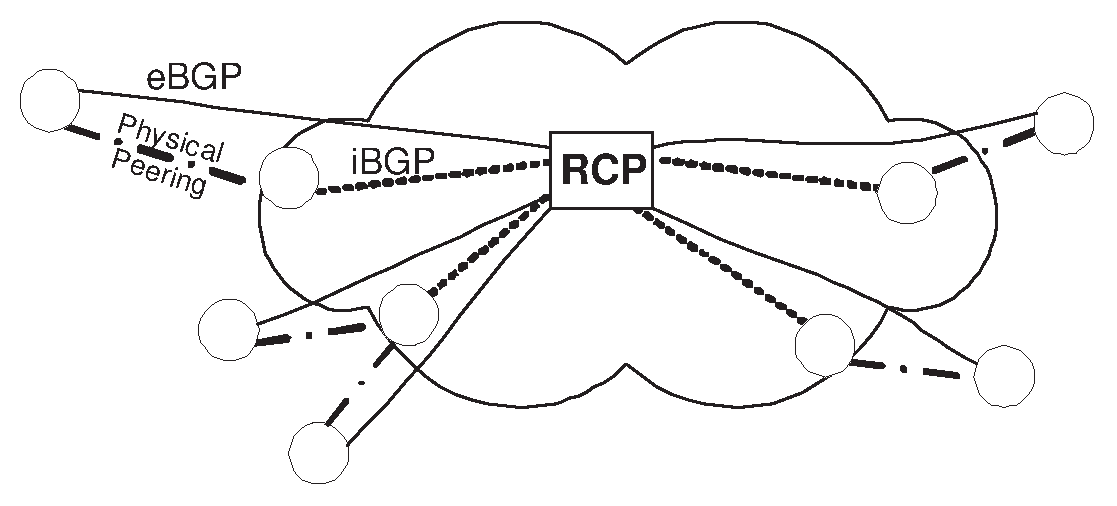
\epsfig{file=rcp/figures/ebgp.eps, width=0.6\linewidth}
\caption[The second phase of RCP deployment]{The second deployment phase
of RCP operates in a similar manner 
  as the first phase, but now RCP itself has eBGP sessions
  to routers in other ASes, rather than relying on border routers
  to learn routes from other ASes and apply local policies.}
\label{fig:ebgp}
\end{figure}


In the first deployment phase, the AS's border routers continue to
exchange routes with neighboring domains.  The AS's border routers still apply
local import and export policies and forward a single best route for
each prefix to RCP.  In the second stage, RCP exchanges routes
directly with the border routers in other ASes, as shown in
Figure~\ref{fig:ebgp}.  Neighboring ASes must modify the
configuration of their eBGP sessions to peer with RCP, rather than
with individual routers.\footnote{Each router on the path
  between RCP and routers must also have routes for both endpoints.
These routes can be established by injecting routes for the endpoints
into the routing protocol or by configuring static routes.}
This change only involves changes to the router {\em configuration}, not the
underlying hardware or software, and it
offers significant benefits because (1)~RCP has access to {\em all\/}
routes learned via eBGP from other ASes, (2)~all routing policies
for the AS are applied directly at the RCP, and (3)~the border routers do
not need any BGP configuration beyond their iBGP session to RCP. 
This phase of RCP significantly simplifies network management.

{\bf Simpler routing configuration.}  With all of the eBGP-learned
routes in one place, the configuration of the routing policies can
reside entirely at the RCP.  Rather than using BGP communities to tag
routes at one router to ensure the correct handling at another router,
RCP can classify and select the routes itself.  For example, suppose
eBGP routes learned from one peer should not be advertised to another.
RCP could maintain a local registry of peer and customer AS
numbers and ensure that routes where the neighboring AS is a peer AS
are not advertised via eBGP sessions to other peer ASes.  In today's
routing infrastructure, the auxiliary information about peer and
customer ASes would be expressed indirectly (\ie, in the import
policies that tag the routes learned on certain eBGP sessions and
export policies that filter routes based on these tags).  With the RCP
performing all routing decisions, this type of decomposition is unnecessary.

{\bf Network-wide traffic engineering.}  In the second phase, RCP has
access to {\em all\/} of the eBGP-learned routes, not just the best
paths selected by the border routers.  With complete control over the
selection of paths, RCP can disregard the unwieldy BGP
decision process.  RCP can influence
the routing decisions of various routers directly, without 
meddling with local preference settings at individual routers.  Rather
than generating complex import policy rules that manipulate the
local preference attribute, RCP could explicitly decide which path
each router should select for any destination prefix.  In
addition to comparing the eBGP-learned routes, RCP could base routing
decisions on
auxiliary information such as measured traffic volumes, performance
statistics (\eg, observed packet loss), and commercial
relationships with neighboring domains (\eg, the pricing model).
%Directly incorporating these metrics into the
%routing protocol is a more appealing way to engineer
%the flow of traffic in the network than trying to find a suitable
%setting of distributed configuration parameters~\cite{Feamster2004}.
%It could, for example, decide to ignore AS path length as a step in
%the decision process, or group routes with different AS path lengths
%into the same equivalence class to assist with traffic
%engineering~\cite{Feamster2003e}.

{\bf Intelligent route-flap damping.}  Many BGP update sequences
are caused by routers performing ``path exploration'': upon learning of
a route's 
withdrawal from a neighboring AS, a router will readvertise its second
best path until it receives the corresponding withdrawal for that path, and
so on.  RCP can prevent route-flap damping from discarding an
otherwise stable route.  Rather than having routers implement route-flap
damping independently, RCP could damp routes on behalf of routers in
the AS based on a network-wide view of the eBGP-learned routes.
Additionally, RCP could determine when advertisements appear to stem
from path exploration and use this information to delay readvertisement,
thus preventing routers in neighboring ASes from receiving a flurry of
transient advertisements during path exploration.

{\bf Coalescing routing table entries with customized aggregation.}
Networks often advertise multiple subnets in the same address block to
balance the flow of traffic over several incoming links, which can
lead to large routing tables and a larger number of BGP update
messages.  An individual router cannot typically safely aggregate
subnets with the same next-hop, because another router in the AS may
need to treat the subnets 
differently.  As 
such, operators are often conservative in aggregating routes to
prevent unintentional blackholes and forwarding loops.  Giving RCP
control over which BGP routes are sent to each router permits
more aggressive aggregation.  For example, if RCP
discovers that the BGP routes for 12.1.2.0/24 and 12.1.3.0/24 at some
router will use the same outgoing interface, it can send a single
12.1.2.0/23 route to the router, which can substantially reduce the
memory requirements for the routing and forwarding
tables.\footnote{An individual router can coalesce subnets when
constructing its local {\em forwarding\/} table~\cite{draves99}, but
this approach does not reduce the size of the BGP routing table or the
number of BGP update messages.}  (Note that RCP can send an
aggregated route to a router even if the two initial routes have {\em
different} AS paths, since the individual routers no longer act on
this information.)  This technique can also reduce the
number of BGP updates, since
many BGP routing changes affect attributes such as AS path, community,
and MED that do not affect forwarding.

%ASes often advertise more specific prefixes to load balance incoming
%traffic; for example, an AS might split a ``$/19$'' prefix into two
%$/20$ prefixes and advertise each smaller prefix on a different link.
%An AS might also divide its prefix into smaller prefixes according to
%geography.  These more specific prefixes can provide ISPs more
%efficient routes to destinations, but they also inflate routing table
%size.  For example, the CIDR report suggests that more aggressive
%aggregation for prefixes that have the same AS paths could reduce
%routing table size by about 40,000 prefixes~\cite{www-cidr}.  An AS's
%RCP can recognize when a router in the AS would select the {\em same}
%route for two contiguous smaller prefixes and aggregate the two
%smaller prefixes into a single routing table entry on that router.

%{\bf Diagnostics.}
%% XXX Punt this paragraph?  Too confusing?
%% An RCP can also enable an AS to perform better diagnostics by providing
%% all eBGP-learned routes in a centralized location.  For example, an AS
%% typically wants to verify that a neighboring AS with which is has a
%% commercial ``peering'' relationship is advertising routes with
%% equally good attributes at all peering locations between the two ASes.
%% Checking this constraint in today's routing architecture is challenging
%% because the routes that one AS advertises to another are distributed
%% across multiple routers.  
%% %Monitoring the best routes from these routers
%% %via iBGP is difficult because some of these routers may choose best
%% %routes from different peers.  Looking at routing table dumps will show
%% %what routes each router hears, but because of the asynchrony, mismatches
%% %in routes as seen in routing tables may reflect inconsistencies due to
%% %timing, rather than actual inconsistent advertisement.  
%% An RCP makes
%% these problems go away because all eBGP routing information is
%% maintained at a logically centralized place.


\paragraph{Redefinition of Inter-AS Routing}\label{sec:interas}

%In the second phase, eBGP is a legacy routing protocol for exchanging
%BGP routes with ASes that do not have RCPs of their own.  
In the third
phase, multiple ASes with RCPs can exchange interdomain routing
information directly through their RCPs, as previously shown in
Figure~\ref{fig:interas}. As in the first
two phases, RCP makes routing decisions on behalf of the
routers in its AS.  
%In the simplest scenario, multiple ASes belonging
%to the same institution use RCPs to coordinate their routing
%decisions, a provider's RCP can coordinate with a customer's RCP to
%offer new network services.  
%Ultimately, we envision each AS having
%its own RCP.  
RCP could simply use eBGP to exchange routing
information, but exchanging routes with eBGP is not strictly necessary.
RCP could also enable ASes to better coordinate when 
diagnosing routing problems and selecting paths.

{\bf Better network diagnostics and troubleshooting.}  RCP could
provide diagnostic information to a neighboring AS (or even remote ASes)
upon request.  Network operators regularly send email to
mailing lists (\eg, NANOG) to ask other operators about possible
reachability problems and diagnose problems as they arise.  With RCPs
deployed in many ASes, the collection of RCPs could be treated as a
distributed database of routing information, where each AS maintains a
portion of and provides a query interface to that
information~\cite{Teixeira2004}. 
An AS
could allow other ASes to query the routes that it has learned from
other ASes for debugging (\ie, using RCP query interface as a
sort of master ``looking glass'' server for the entire AS) or
verification~\cite{Feamster2003b} (\eg, verifying an AS path by
asking other ASes along that path if they have learned corresponding
route).
%
Of course, the diagnostic information need not be limited to BGP
data.  For example, RCP could maintain information
about intra-AS topology changes, link congestion, and performance
statistics to help explain disruptions in end-to-end performance.

{\bf New interdomain routing protocols.}  RCP
enables a variety of proposals for fundamental changes
to interdomain routing.  Recent proposals have advocated
modifying the way the interdomain routing protocol selects and
propagates routes. For example, a new routing protocol could attach
prices to advertised routes~\cite{Feigenbaum2002} or explicitly
support inter-AS negotiation to select the routes~\cite{mahajan2005}.
RCPs could also base their routing decisions on measured
end-to-end performance, as proposed in work on overlay
networks~\cite{Andersen01} and even make this performance information
available to end-host overlays through appropriate
interfaces~\cite{Nakao2003}.
%
Other proposals have suggested ways to improve security by performing
path authentication~\cite{Subramanian2004} or origin
authentication~\cite{Aiello2003}.  Until now, many of these proposals
have had no feasible deployment path because they require fundamental
protocol changes and would not be backwards compatible with the
installed base of routers.  RCP allows the deployment of new routing
protocol changes without modifying or replacing the existing infrastructure.

%Pairs of ASes must sometimes coordinate their policies to achieve
%certain traffic engineering tasks.  In Section~\ref{sec:principles}, we
%described, the complications involved in expressing bilateral
%interdomain routing policies such as backup and load balance.  RCP
%could simplify this type of policy negotiation by (1)~allowing
%high-level policies like backup to be negotiated in-band (\ie, in the
%routing protocol itself) and (2)~allowing complex traffic policies to be
%implemented without indirect, low-level tweaks of routing protocol
%attributes.

%In addition to previously proposed protocol alternatives, an RCP-based
%routing architecture enables other types of fundamental changes to the
%routing protocol.  For example, the RCP could exchange performance
%information (\eg, path level performance information that overlays
%currently perform~\cite{Andersen01}, information about resource
%availability, etc.) that could help inform routing decisions.

%\subsection{Challenges Introduced by RCP}\label{sec:weaknesses}

%The RCP architecture potentially introduces limitations and weaknesses;
Separating routing state from the routers can potentially introduce
robustness, scalability, speed, and consistency problems.  The RCP
architecture must address these challenges to be viable.  In this
subsection, we briefly highlight these issues and sketch
possible solutions to these problems.  We are
addressing these problems in greater detail in our current work,
and we are implementing a prototype of RCP using OSPF and BGP
data from AT\&T's domestic IP backbone~\cite{caesar2004}.

It might seem that moving complexity out of the routers
into RCP creates new problems because of the additional flexibility
in path assignment and because we are adding a component to the routing
system.  However, management systems and verification tools
for BGP configuration already exist today, but they are more complicated
and constrained because they must work around the artifacts of today's
routing system.  Thus, adding RCP to the routing system does not
really constitute ``more functionality''; rather, RCP moves
routing functionality to a part of the system where complexity can be
better managed.

%We briefly highlight some of the potential challenges presented by the RCP
%architecture and our proposed solutions to these problems.  We discuss
%these problems in more detail in an accompanying technical
%report~\cite{caesar2004}. 


 {\bf Robustness.} To avoid introducing a single point of failure, RCP
  should be distributed across multiple {\em RCP servers} (RCSes).
  These servers must maintain a consistent view of the available routes
  to ensure that all routers receive consistent, loop-free paths.  The
  RCSes must employ a protocol that recognizes when an AS becomes
  partitioned and guarantees that each partition receives routing
  information that is consistent within its partition.  We are currently
  studying the types of inconsistencies that can result from various
  combinations of partitions.  Our preliminary results suggest that
  even if a network is partitioned, RCSes in separate partitions cannot
  create a forwarding loop.  This result follows from the fact that
  network partitions are caused by partitions of the IGP (\eg, OSPF)
  topology, and RCSes rely on the IGP to exchange routes with each other
  and with BGP routers.  Thus, a protocol that elects an RCS for
  each partition guarantees correct, loop-free forwarding.


%%   Our preliminary results suggest that,
%%   because network partitions result from a partition in the internal
%%   routing protocol (\eg, OSPF), the types of partitions that can cause
%%   RCP-induced forwarding loops are not generally possible and that a
%%   protocol that allows each RCS to determine which RCS learns the most
%%   candidate routes within its partition (and, thus, which RCS is the
%%   ``master'') suffices to guarantee correct, loop-free
%%   forwarding.
%\footnote{Forwarding loops
%  resulting from inconsistent route advertisements require two RCP
%  servers with different routing choices to assign routes to the same
%  set of routers.  In other words, such inconsistencies require RCP
%  servers in two partitions $A$ and $B$ to share some set of routers,
%  but $(A \cup B - A \cap B) \neq \phi$.  We have shown that, if $(A
%  \cup B - A \cap B) \neq \phi$, then the RCP servers in $A$ and $B$
%  cannot be partitioned.}.


%We believe that existing state machine replication
%  or primary/backup schemes may be applicable.

 {\bf Scalability.} RCP must be able to handle thousands of eBGP
  sessions and hundreds of iBGP sessions, each with thousands of routes.
  Today's high-end desktop machines satisfy the memory and computational
  requirements for RCP.  In our current work, we are exploring ways to
  distribute RCP functionality across many physical machines.  One
  design idea we are currently pursuing involves dividing the RCP into a
  {\em BGP engine}, which is responsible for establishing the (possibly
  large number of) BGP sessions to routers within the AS (and,
  ultimately, across ASes) and whose sole responsibility is state
  management; and an {\em RCP engine}, which receives the routing
  information from the machines running BGP engines and implements the
  logic that we have discussed (\eg, path computation,
  configuration management, maintaining consistency, etc.).  
  

 {\bf Convergence speed.} RCP must compute routes using BGP and
  IGP information for every router in the AS and propagate the results
  of this computation in a timely fashion as BGP and IGP topologies
  change.  Because RCP is an active participant in both the BGP and
  IGP protocols, delays due to message passing should be no worse than
  in today's routing architecture.

 {\bf Transient inconsistencies.}  Transient inconsistencies might occur
  if routers do not receive updates from RCP in a certain order. For
  example, if a router's path to a destination includes routers for
  which RCP has already assigned a new path, transient forwarding
  loops could result.  Although this pathology is likely no worse than the
  transient loops that occur during iBGP convergence today, it deserves
  further attention.  In the future, routers might be modified to
  support a ``commit'' operation to allow for all routers along a path
  to execute an update at the same time.



%

XXX remove
Scaling problems exist not only within a single AS, but also between
groups of ASes.  The route arbiter project proposed placing route
servers at exchange points~\cite{Govindan1998} to obviate the need for a
full mesh eBGP topology (\ie, at the exchange point) by applying policy
once at the route server.  This architecture facilitates centralized
application of BGP routing policies at a single exchange point.  In
Section~\ref{sec:rcp}, we present RCP, which primarily addresses how to
scalably disseminate routes {\em within} a single AS.  In some ways, RCP
can be viewed as an analog to route servers~\cite{Govindan1998} for
intra-AS route dissemination: whereas route servers were used to reduce
the number of eBGP sessions from $O(n^2)$ to $O(n)$, where $n$ is the
number of ASes at an exchange point, RCP reduces the number of iBGP
sessions from $O(n^2)$ to $O(n)$, where $n$ is the number of routers in
a single AS.  Because RCP separates the logic of route selection from
the physical routers, it is conceivable that it could also used as a
platform for developing new mechanisms for exchanging routes between
pairs or groups of routers. 


Ultimately, RCP can facilitate innovation because it allows the logic of
route selection to be located in a system that is separate from the
infrastructure that is responsible for forwarding data traffic.  Moving
routing into a logically centralized (albeit replicated) system creates
more flexibility in how routes are exchanged between RCP nodes in
neighboring ASes: RCP nodes in adjacent ASes could use BGP to exchange
these routes, 
although they could conceivably use any protocol.  RCP could also expose
more information about the routing topology to applications such as
overlay networks, as well as give these networks more control over the
IP-level routes that are actually used.

Moving routing functionality into a system like RCP is not the only way
to separate routing from forwarding: others have advocated removing
routing from the AS entirely by moving routing complexity to end hosts,
which query route servers to discover routes~\cite{Lakshminarayanan2004,
Yang2003}.  Although these projects share our goal of separating routing
complexity from the infrastructure, RCP has the added benefit of
simplifying intra-AS routing.  Recent work has also proposed working
around the existing infrastructure, using an overlay to improve BGP's
robustness~\cite{Agarwal2003, Goodell2003}.


\subsubsection{Provide direct control over traffic}

Much research, both in Chapter~\ref{chap:sandbox} and in previous
work~\cite{Feldmann2000}, has focused on developing predictive models of
network-wide routing, typically to assist network operators in traffic
engineering. A system like RCP can provide {\em real-time control\/} of
BGP routes rather than modeling the BGP routes in today's routing
system.  That is, rather than trying to infer the outcome of BGP route
selection or otherwise monitor the routing protocol (as many existing
systems do~\cite{www-ipsumnetworks,www-packetdesign, Shaikh2004}), RCP
can {\em control} the outcome, thus directly controlling how traffic
flows.

Although RCP provides direct control over traffic, it does not provide
any facilities for helping operators determine {\em how} that traffic
should be controlled.  Similarly, Chapter~\ref{chap:sandbox} presented
algorithms that help network operators predict the effects of
configuration changes on the flow of traffic through the network, but
these algorithms do not help network operators actually discover a
routing configuration that achieves their intended objective (\eg,
relieving persistent congestion, minimizing congestion on peering links,
etc.).  Unlike {\em intra}domain routing optimization, for which there
are existing tools and algorithms to help operators tune
parameters~\cite{www-cariden-mate,Feldmann2000}, {\em inter}domain routing is
much more difficult to optimize: the search space is much larger, and
local configuration changes can have global effects that alter the
traffic volumes coming {\em to} that AS from neighboring ASes.  Our
previous work proposes some guidelines for helping network operators
make configuration changes that are less likely to cause unpredictable
effects~\cite{Feamster2003e}, but the design techniques for efficiently finding
optimal (or even ``good'') configuration settings remain open.


\subsubsection{Avoid manipulable routing objects}

Recall from Chapter~\ref{chap:rlogic} that we considered a destination
$d$ to be an immutable ``handle'' for a route that referred to a set of
endpoints; we cited IP prefixes as the destination $d$ in
the case of Internet routing.  Unfortunately, prefixes are {\em not}
immutable: a router in one AS can {\em aggregate} IP prefixes that are
contiguous in 
the address space taking two routes, $(d_1 \rightarrow v_i)$ and $(d_2
\rightarrow v_j)$ and combining them into a single route, $(d
\rightarrow v_k)$, such that any packets destined for endpoints in
either $d_1$ or 
$d_2$ will be forwarded according to the route $(d\rightarrow v_k)$.
This creates complications for the definition of an induced path
(Definition~\ref{defn:ipath}), since a route to any endpoint by be
induced by routes for different destination handles at different
routers.

\begin{figure}
\centering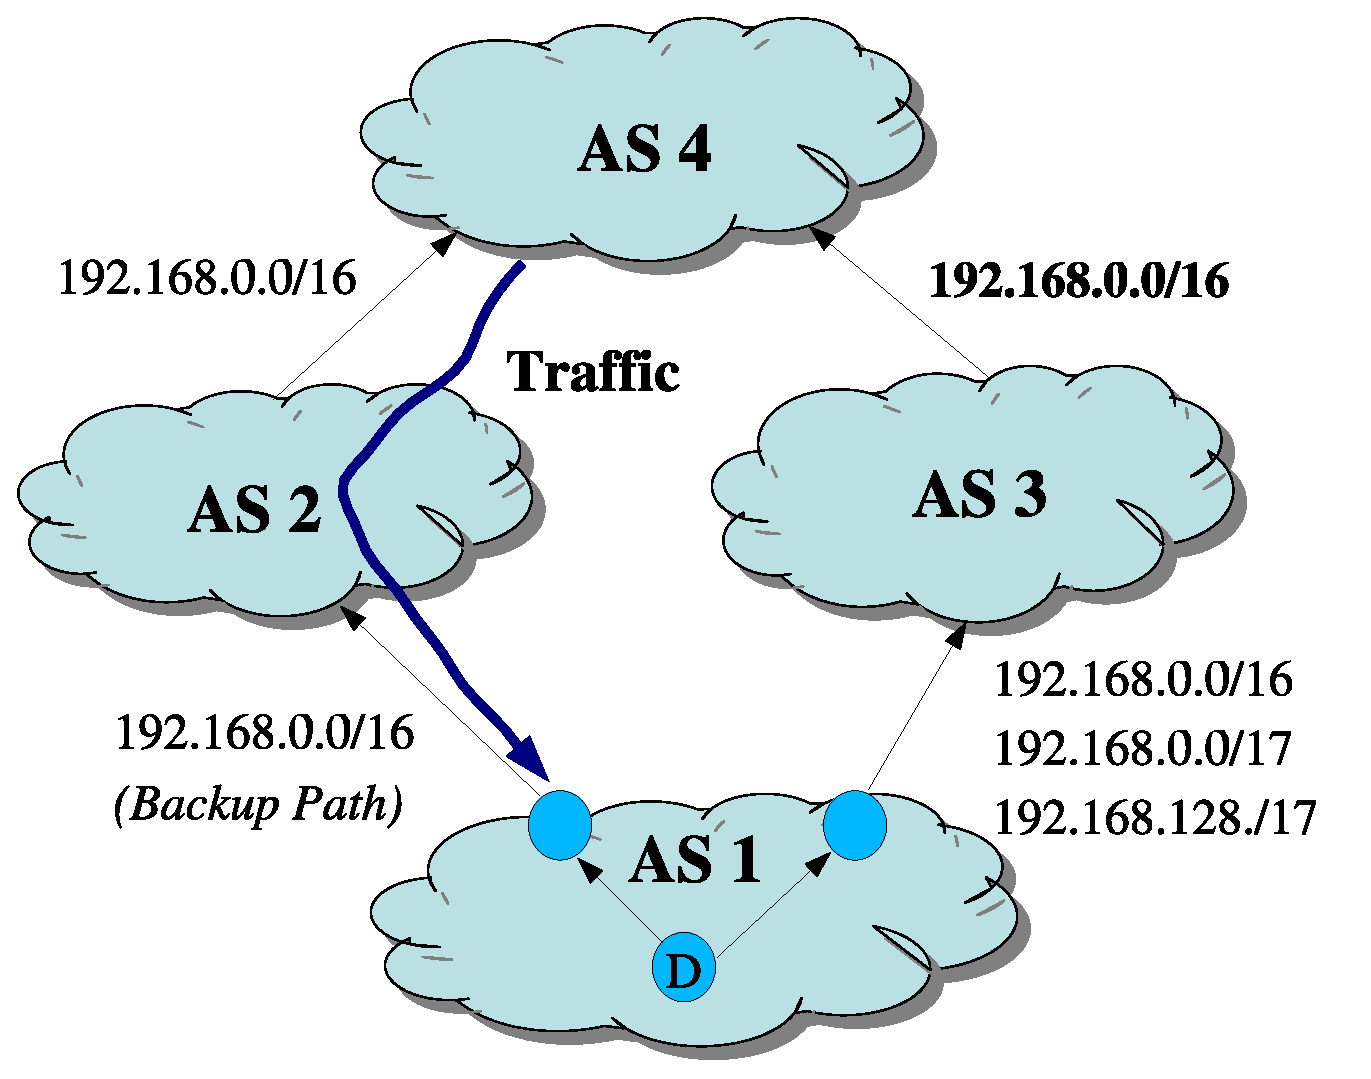
\epsfig{file=figures/aggregate.eps, width=0.65\linewidth}
\caption[How aggregation can interfere with an AS's attempt to control
  inbound traffic.]{Aggregation can interfere with an AS's attempt to
  control inbound traffic.  In this example, AS~1 announces more
  specific routes to AS~3 in an attempt to have inbound traffic enter
  via that AS.  AS~3, on the other hand may aggregate (or simply filter)
  those more specific routes to save routing table space, thus
  interfering with AS~1's intent.}
\label{fig:aggregate}
\end{figure}

Not only do these manipulable routing objects create problems for reasoning
about properties of the routing protocol, but they also create practical
problems.  For one, they create a tension between control over inbound
traffic and scalability.  ASes typically exploit the fact that routers
will forward traffic based on the longest matching IP prefix in the routing
table and send more specific routing information along links where it
wishes to attract traffic.  This technique allows an AS to control how
traffic reaches its AS from 
other places on the Internet.  On the other hand, to control routing
table size, some ASes may combine multiple more specific routes into a
single shorter route using a process called aggregation.  Aggregation
dramatically reduces routing table size because Internet addressing is
typically hierarchical.  Unfortunately, aggregating more specific
prefixes can also interfere with an ASes attempt to control how traffic
reaches its network, as shown in
Figure~\ref{fig:aggregate}~\cite{id-path-validation}.  Thus, ASes must
either aggregate routes at the risk of interfering with the traffic
engineering goals of other ASes (the common practice
today~\cite{nanog-prefix-aggregation}) or maintain larger routing tables
without receiving compensation for the incurring the extra overhead.

Finally, recent work has observed that, because IP prefixes can be
manipulated by routers in other ASes, they often do not accurately
reflect a set of destinations 
that is atomically either reachable or
unreachable~\cite{Freedman2005}. This characteristic can cause
violations of route validity (Definition~\ref{defn:rv}) when a portion
of endpoints contained within some destination become unreachable but
the route advertising the IP prefix for those endpoints is not
withdrawn.

In light of these problems presented by aggregation, one reasonable
design principle for future Internet routing systems may be to make the
destination that is referred to by a route an 
immutable property of the route, as a recent proposal has
suggested~\cite{Vutukuru2005b}. 

%% Even if a router makes the same routing decision for two contiguous
%% prefixes, it typically cannot aggregate those routes because it does not
%% know if other routers that learn BGP routes from this router might
%% select different routes for the separate prefixes.  

%% AIP as possible answer?








\subsection{Consider the effects of adversaries on correctness
and predictability}
\label{sec:concl:security}

This dissertation addresses the challenges for correctness and
predictability that are introduced unintentionally.  A growing threat to
the Internet routing infrastructure, however, is that posed by
adversaries.  For example, malicious parties may attempt to inject false
routing information in an attempt to divert or blackhole traffic.
Routing security has been studied in some detail~\cite{perlman88}, but
{\em interdomain} routing security is particularly difficult because
interdomain routing must support complex policy.  In addition to
securing routing information, the infrastructure should also ultimately
provide guarantees about where the traffic actually goes---in other
words, whether the {\em induced path} (Definition~\ref{defn:ipath},
Chapter~\ref{chap:rlogic}) actually corresponds to the information about
the path that is carried in the route.


\subsubsection{Control-Plane Security}

Attacks against the control plane have received considerable attention
in recent years.  The IETF has established a working group in routing
protocol security, RPSEC~\cite{rpsec-wg}; recent drafts have addressed
threats to the Internet routing system and BGP and outlined security
requirements~\cite{id-routing-threats}.  BGP does not provide any
support for controlling route announcements.  Securing the control plane
boils down to two tasks: {\em origin authentication}, which verifies
that the AS that is announcing (``originating'') the prefix actually has
legitimate ownership over the address space for that prefix; and {\em
path authentication}, which verifies that the sequence of ASes that the
routing advertisement traversed corresponds to the sequence of ASes in
the AS path.

Various proposals provide either origin authentication~\cite{id-sobgp},
path authentication~\cite{Hu2004:spv}, or both~\cite{kent2000b}.
Unfortunately, these schemes require the existence of a public
key infrastructure (PKI), a central authority that manages key
distribution, ownership, and revocation; PKIs are cumbersome and
difficult to 
maintain.  Thus, developing a routing protocol that automatically
verifies the ownership of some address space without requiring a
centralized, trusted verification or lookup infrastructure remains an
important unsolved problem.

Even an Internet routing architecture that provides both origin and path
authentication still does not enable an AS to verify that the route it
receives is one that it {\em should be receiving}.  That is, while they
allow an AS to verify that a route announcement traversed a particular
sequence of ASes, they do not provide any mechanism to allow an AS to
verify that the sequence of ASes is one that is sensible.  Answering
this question is critical for routing security.  If an AS has no way to
determine whether a sequence of ASes is sensible, then it is possible
for a single malicious organization to establish a new AS and have that
AS buy transit from the upstream AS of a source and destination,
respectively.  An important unsolved problem involves characterizing the
types of bogus routes that an AS can detect with the limited information
available today, as well as determining the additional information that
should be added to the routing protocol that could assist this detection
without 
revealing sensitive business relationships.


\subsubsection{Data-Plane Security}

Even if an AS could verify that the routes it receives were authentic
and policy-compliant, it still has no way to verify that packets
actually traverse the same ASes as those in the route's AS
path~\cite{Mao2003}.  We note that the AS path was never intended as an
indication of the ASes that traffic will actually traverse.  Rather, the
AS path was only
ever intended for loop detection (\ie, so that an AS would not
readvertise a route that it had already learned) and as a coarse metric
for choosing shorter routes over longer ones.  Nevertheless, providing
some guarantees over where traffic will (or won't) travel appears to be
a desirable goal for Internet routing.  Allowing an AS or end host to
verify that a route's AS path matches the actual forwarding path, or,
more generally, allowing it to ascertain the sequence of ASes that
traffic to or from some destination traverses are important capabilities
that any future Internet routing system should provide.  

%% While restricting route propagation is a reasonable way to restrict
%% unwanted traffic, a malicious entity can always try to ``dump'' traffic
%% for a certain destination on any advertised link, in the hope that the
%% router will carry traffic to that destination anyway.  A router should
%% reject packets destined for hosts with no corresponding advertised
%% route.  More generally, a router should reject packets from sources that
%% should not have a valid route through this router to the destination.
%% Deploying packet filters only at routers in large ASes in the Internet
%% ``core'' could eliminate most of these packets~\cite{Park2001}, but an
%% AS must be able to construct these filters in the first place, which
%% would require discovering the routes from the source to that AS.
%% \begin{itemize}
%% \itemsep=-1pt
%% \item {\em Dynamic packet filter construction.} How can an AS
%%   determine the source and destination addresses it
%%   should see on packets arriving on a link?~\footnote{This
%%   question has a dual for {\em route\/} filters in the 
%%   control plane.} 
%% \end{itemize}


\section{Concluding Remarks}\label{sec:final}

%% Muse about how awesome the correctness specification is and how it can
%% be used to analyze all of these cool new features and additions.  Now,
%% it's just our job to come up with those features!

This dissertation has (1)~presented a correctness specification for
Internet routing; (2)~developed tools and techniques to check for
violations of this correctness specification in real-world routing
configuration; (3)~exploited the correctness specification to design
algorithms that predict the outcome of BGP route selection for the set
of routers within an AS; and (4)~derived the first conditions for
guaranteeing a {\em global} correctness property, safety, that do not
require global knowledge of business relationships or topology.  

The current version of the Internet's routing protocol, BGP, has been
deployed for nearly a decade and has been modified and extended numerous
times (\eg, with route reflection).  More striking is the plethora of
proposals that have not been deployed.  In light of these proposals, the
key challenge is to be able to separate the good protocol modifications
from the bad ones and to determine how these various modifications
interact with each other. 
The correctness specification presented in this dissertation facilitates
this type of reasoning. Furthermore, the proactive techniques that this
dissertation has advocated and developed can help resolve the tension
between flexibility and complexity that exists in any complex routing
protocol. 
%proposed routing 
%protocol (or even a modification to BGP, for that matter) will solve the
%problems it claims to solve without introducing new problems of its own.
While we have presented the properties of the correctness specification
in the context of BGP, it is our hope that this specification can serve
as a guide for both evaluating and designing new routing protocols that
explicitly provide correctness and predictability. 


